\documentclass[]{article}

\usepackage[utf8]{inputenc}

\usepackage{eurosym}
\usepackage[
  margin=1.8cm,
  includefoot,
  footskip=10pt,
]{geometry}
\usepackage{graphicx}
\graphicspath{{figures/}}
\usepackage[english]{babel}
\usepackage{url}
\usepackage[colorlinks=true, linkcolor=black, urlcolor=blue]{hyperref}
\usepackage{color}
\usepackage[dvipsnames]{xcolor}
\usepackage{titling}
\usepackage{subfig}
\usepackage[bottom]{footmisc}
\usepackage{titlesec}
\usepackage{chngpage}
\usepackage{calc}
\usepackage{listings}

\definecolor{gray}{rgb}{0.4,0.4,0.4}
\definecolor{darkblue}{rgb}{0.0,0.0,0.6}
\definecolor{cyan}{rgb}{0.0,0.6,0.6}

\lstset{
  basicstyle=\ttfamily,
  columns=fullflexible,
  showstringspaces=false,
  commentstyle=\color{gray}\upshape
}


\setcounter{secnumdepth}{4}


\newcommand{\minit}[1]{\noindent{\small\textbf{ \underline{#1}}}~\\}
\newcommand{\todo}[1]{\par{\color{red} /---| A faire : #1 |---\textbackslash\\}}
\newcommand{\todoIL}[1]{{\color{red}[todo: #1]}}
\newcommand{\wordlink}[2]{\hyperref[#2]{#1~\ref{#2}}}

\titleformat{\paragraph}
{\normalfont\normalsize\bfseries}{\theparagraph}{1em}{}
\titlespacing*{\paragraph}
{0pt}{3.25ex plus 1ex minus .2ex}{1.5ex plus .2ex}

%-- Logos PDG --
\pretitle{
\begin{center}

\begin{figure}[!tbp]
  \centering
  \subfloat{
\includegraphics[width=0.25\textwidth]{UMons_logo.png}}
  \hfill
  \subfloat{
\includegraphics[width=0.25\textwidth]{sciences_logo.png}}\\
\end{figure}
~\newline

}

\posttitle{\end{center}}

\begin{document}

\title{
\vspace{1.6cm}
{\Huge Software Analysis : pacman systems}\\
\vspace{0.5cm}
{\Huge Project report for Software Evolution course}\vspace{1cm}\\
}


\author{
\vspace{1cm}
\huge{Group 3}\\
\Large{BOOSKO Sam}\\
\Large{DECOCQ Rémy}\\
\Large{SCHERER Robin}
}


\date{
\vspace{7.9cm}
Academic Year 2019-2020\\
Master Computers Science, block 2\\
Faculté des Sciences, Université de Mons}

\maketitle          

\thispagestyle{empty}   

\newpage

\tableofcontents
\newpage

%------------- INTRO -------------
\section{Quality analysis of the initial versions}
\subsection{System 1 (BOOSKO Sam)}
\subsubsection{Generalities}

First of all, the structure of the project folder is classic with sub folders, such as:
\begin{itemize}
    \item \textit{src} containing two folders:
    \begin{enumerate}
        \item \textit{main}, all classes for the game (core, gui and movement controller), and
        \item \textit{test} with all unit tests of Junit system.
    \end{enumerate}
    \item \textit{doc}. In this folder, a file, \textit{scenarios.md}, present the goal of the initial project and few scenatios of the game rules. Furthermore, there is another folder, \textit{uml}, containing two uml class diagram files of \textit{uxf} format. These two files describe a simply version of classes (see Figure ~\ref{fig:FactoryWiringClassDiagram} and Figure ~\ref{fig:SinglePlayerGameClassDiagram}).
\end{itemize}

The building system, as demanded in directives, is provided with \textit{Maven}.

\begin{figure}[h]
    \centering
    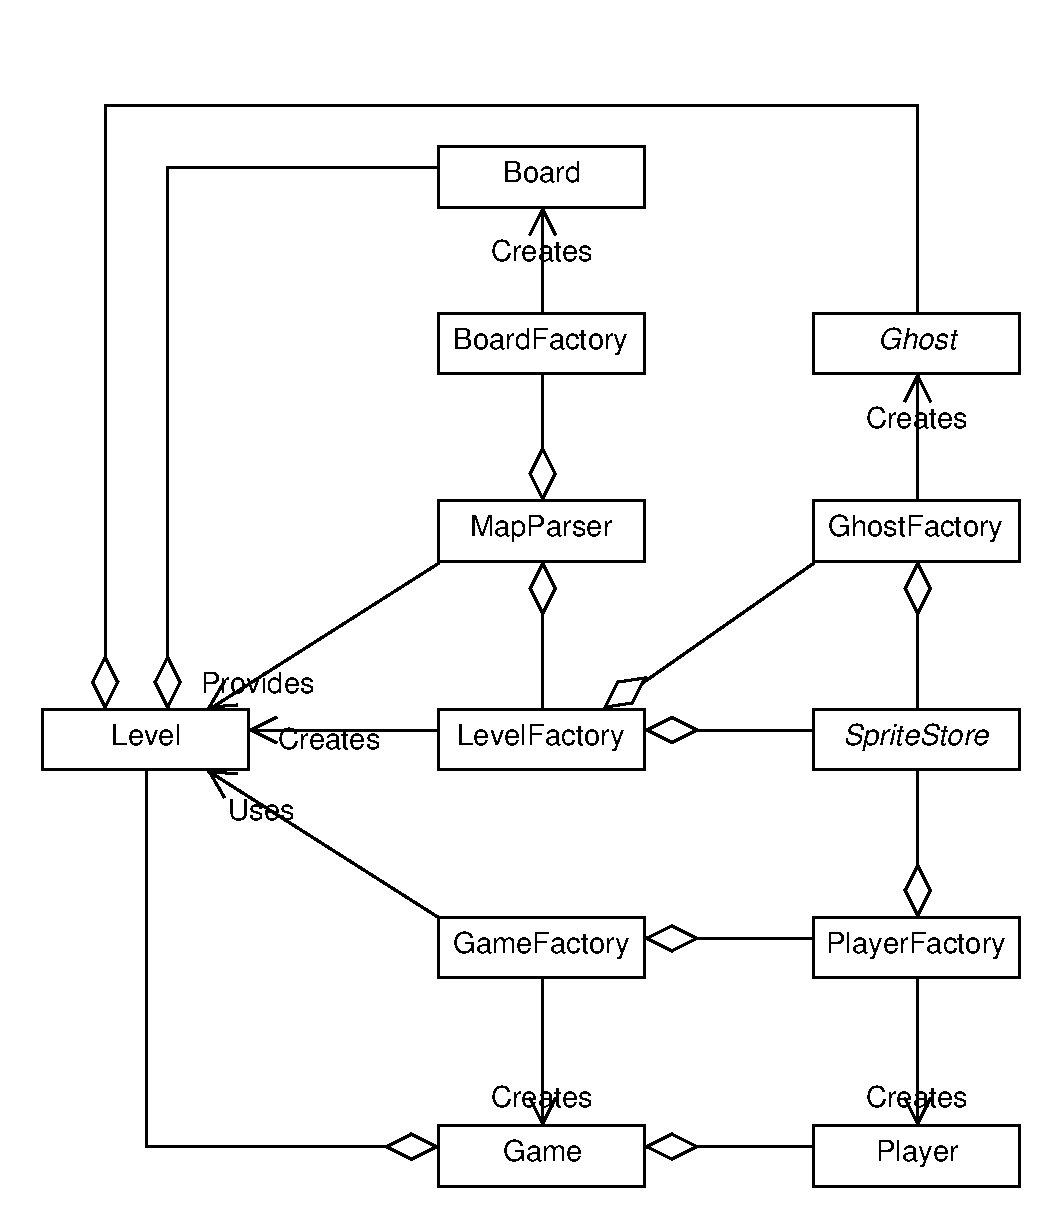
\includegraphics[scale=0.4]{imgs/FactoryWiring.pdf}
    \caption{Factory Wiring Class Diagram}
    \label{fig:FactoryWiringClassDiagram}
\end{figure}

\begin{figure}[h]
    \centering
    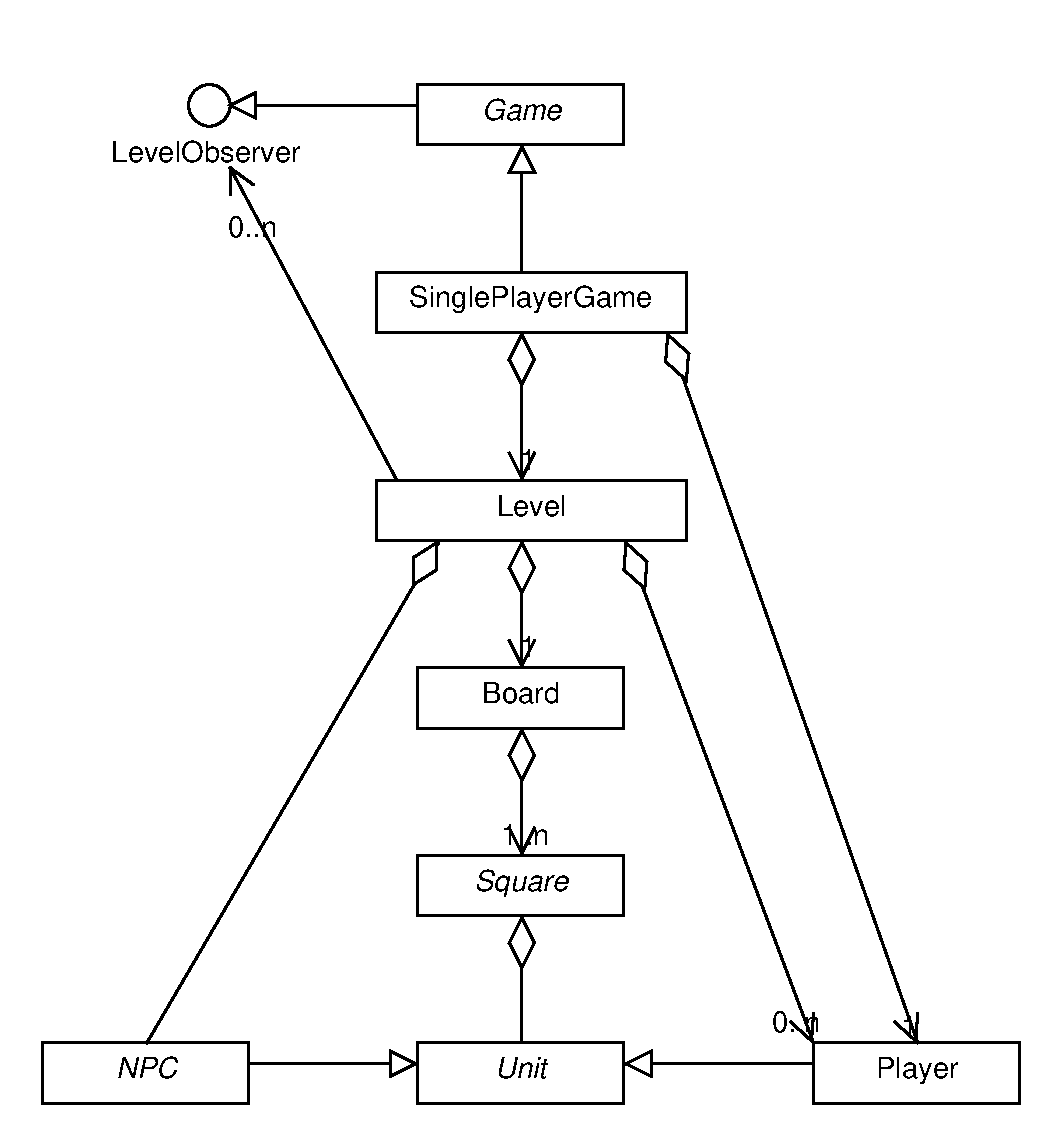
\includegraphics[scale=0.4]{imgs/SinglePlayerGame.pdf}
    \caption{Single Player Game Class Diagram}
    \label{fig:SinglePlayerGameClassDiagram}
\end{figure}

\subsubsection{Static Analysis}

\paragraph{Bad Smells (Designite)}

Designite is a code analyzer which can detect bad smells in a project. Firstly, made for C\# implementation, another version for Java project is provided. Here, designite is used as an \textit{IntelliJ} plugin to have a live visualization during the refactoring and as a "script" to get global information from the project as \textit{csv} files (sample of used file see Table ~\ref{tab:BadSmells}). Furthermore, the output of the "script" gives some information (see Figure ~\ref{fig:DesigniteOutput}), such as the number of cyclic dependency, here 5, the number of magic number, here 39 and also the number of long parameter list, here 8. \\


\begin{table}[h]
    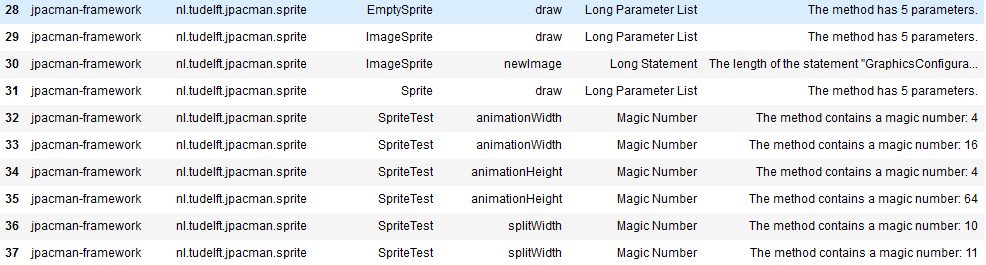
\includegraphics[scale=0.5]{imgs/badSmellsSample.PNG}
    \caption{ImplementationSmells.csv}
    \label{tab:BadSmells}
\end{table}

\begin{figure}
    \centering
    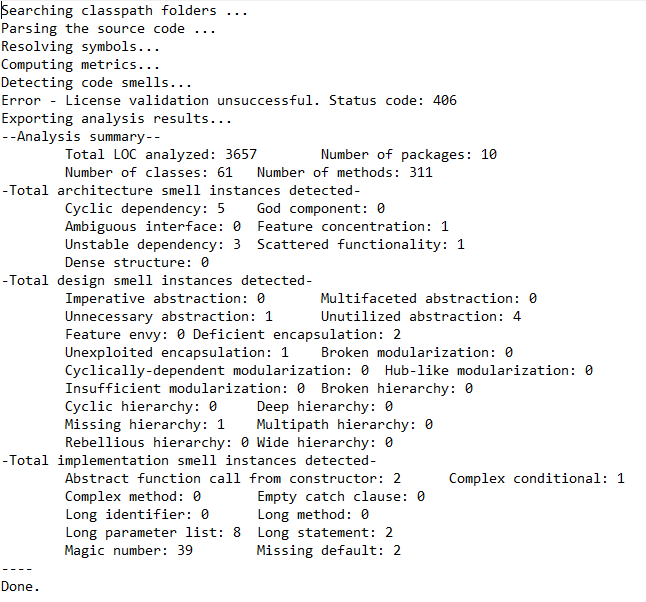
\includegraphics[scale=0.6]{imgs/DesigniteOutput.PNG}
    \caption{Designite Output}
    \label{fig:DesigniteOutput}
\end{figure}

\paragraph{Code Metrics (CodeMR)}

CodeMR is a software which assess a project quality with a static code analysis to help developers or companies to develop better code, products quality. It generates an interactive \textit{html} files to visualize all information assessed as a dashboard.\\

The main page (see Figure ~\ref{fig:CodeMRDashboard}) informs that the project quality is fairly good. Only one problematic class and $9.9\%$ of cohesion lack. \\

By coupling the Figures ~\ref{fig:CodeMRByPackage} and ~\ref{fig:CodeMRDashboard}, we notice that the class \textit{Level} impacts the project quality. The problematic metric, visible from the Figure ~\ref{fig:CodeMRLevelClassQuality}, is the lack of cohesion\footnote{https://www.codemr.co.uk/documents/} defined in the \textit{CodeMR} as "Measure how well the methods of a class are related to each other. High cohesion (low lack of cohesion) tend to be preferable, because high cohesion is associated with several desirable traits of software including robustness, reliability, reusability, and understandability. In contrast, low cohesion is associated with undesirable traits such as being difficult to maintain, test, reuse, or even understand.".

\begin{figure}
    \centering
    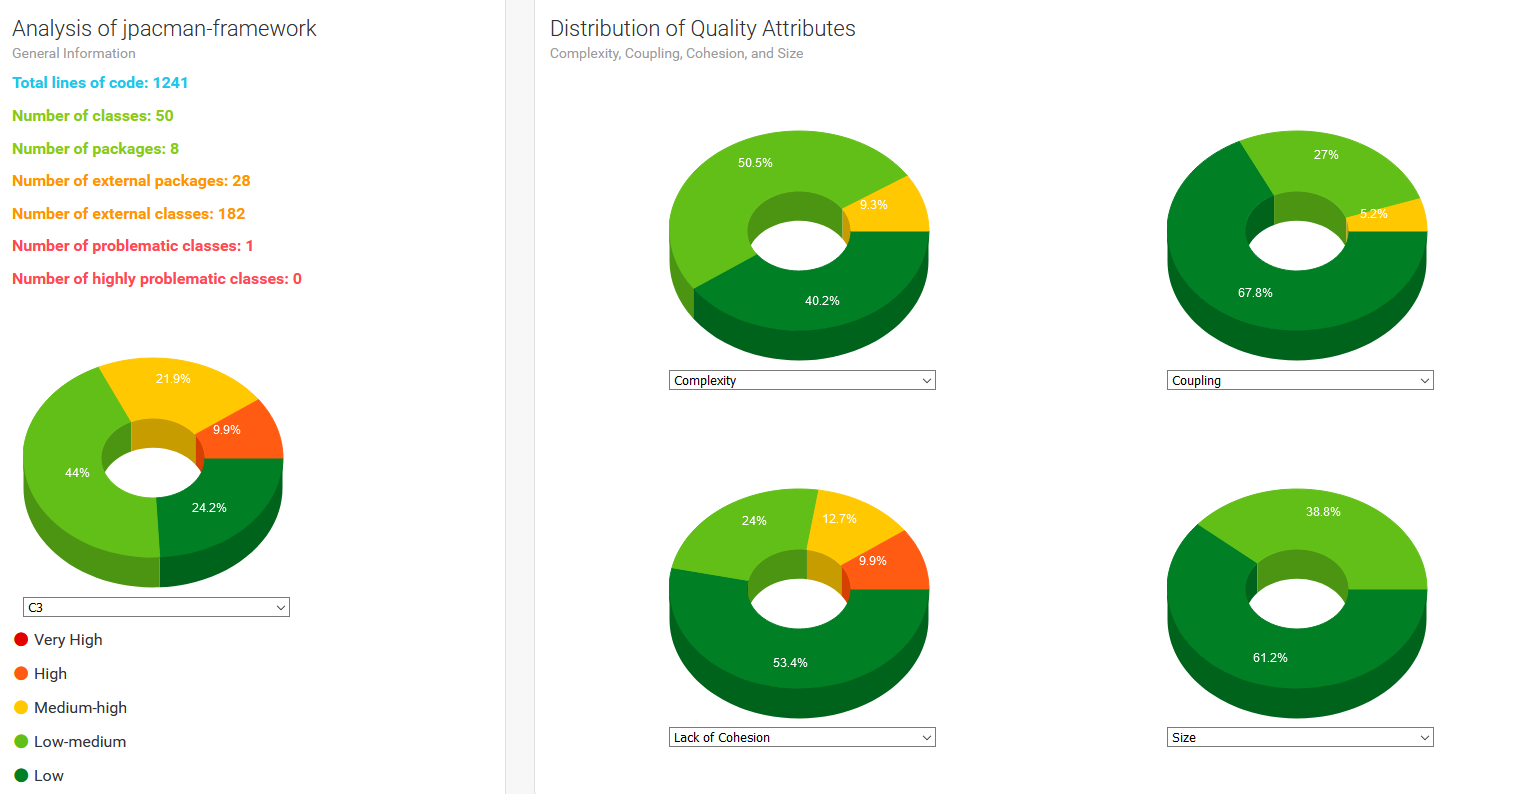
\includegraphics[width=\linewidth]{imgs/CodeMRDashboard.PNG}
    \caption{CodeMR dashboard summarizing health of the system 1}
    \label{fig:CodeMRDashboard}
\end{figure}

\begin{figure}
    \centering
    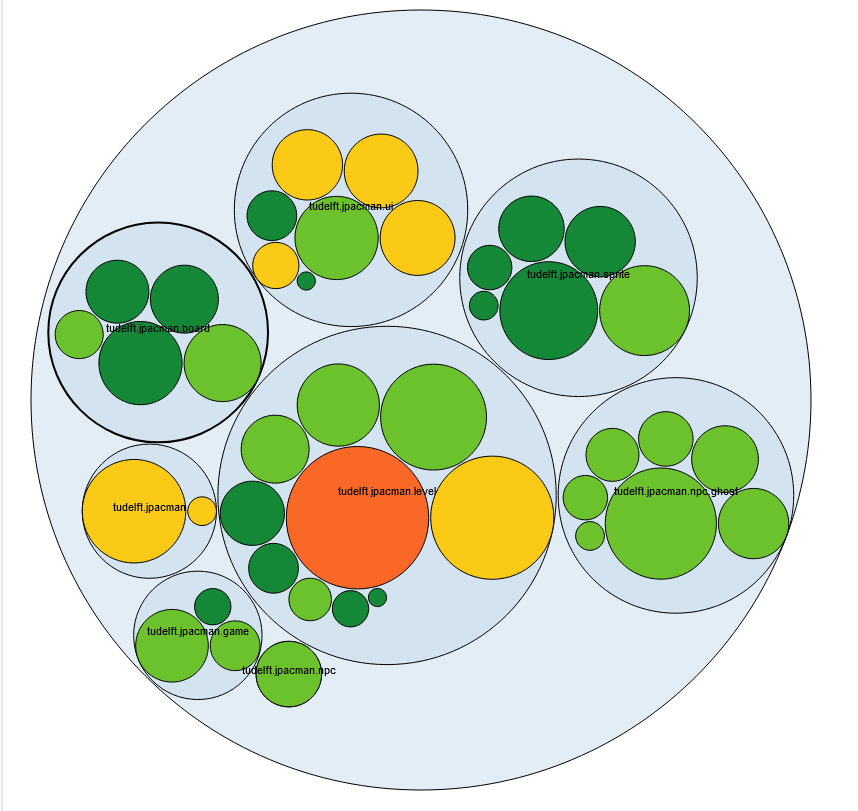
\includegraphics[scale=0.5]{imgs/CodeMRByPackage.PNG}
    \caption{C3 Metric by package for the system 1}
    \label{fig:CodeMRByPackage}
\end{figure}

\begin{figure}
    \centering
    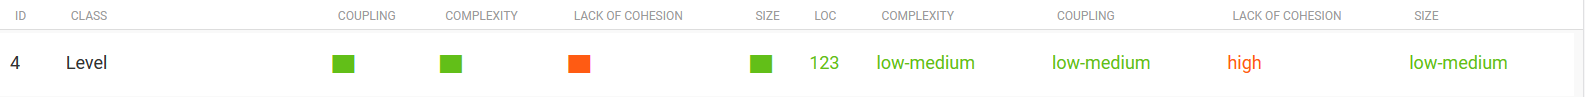
\includegraphics[width=\linewidth]{imgs/CodeMRLevelMetrics.PNG}
    \caption{Metrics of the class Level}
    \label{fig:CodeMRLevelClassQuality}
\end{figure}

\paragraph{Dependencies (IntelliJ analyzer)}

IntelliJ Ultimate version has an analyzer to assess a dependencies matrix (see Figure ~\ref{fig:DependenciesMatrixS1}). We observe, as seen before with Designite analysis, few cyclic dependencies.

\begin{figure}
    \centering
    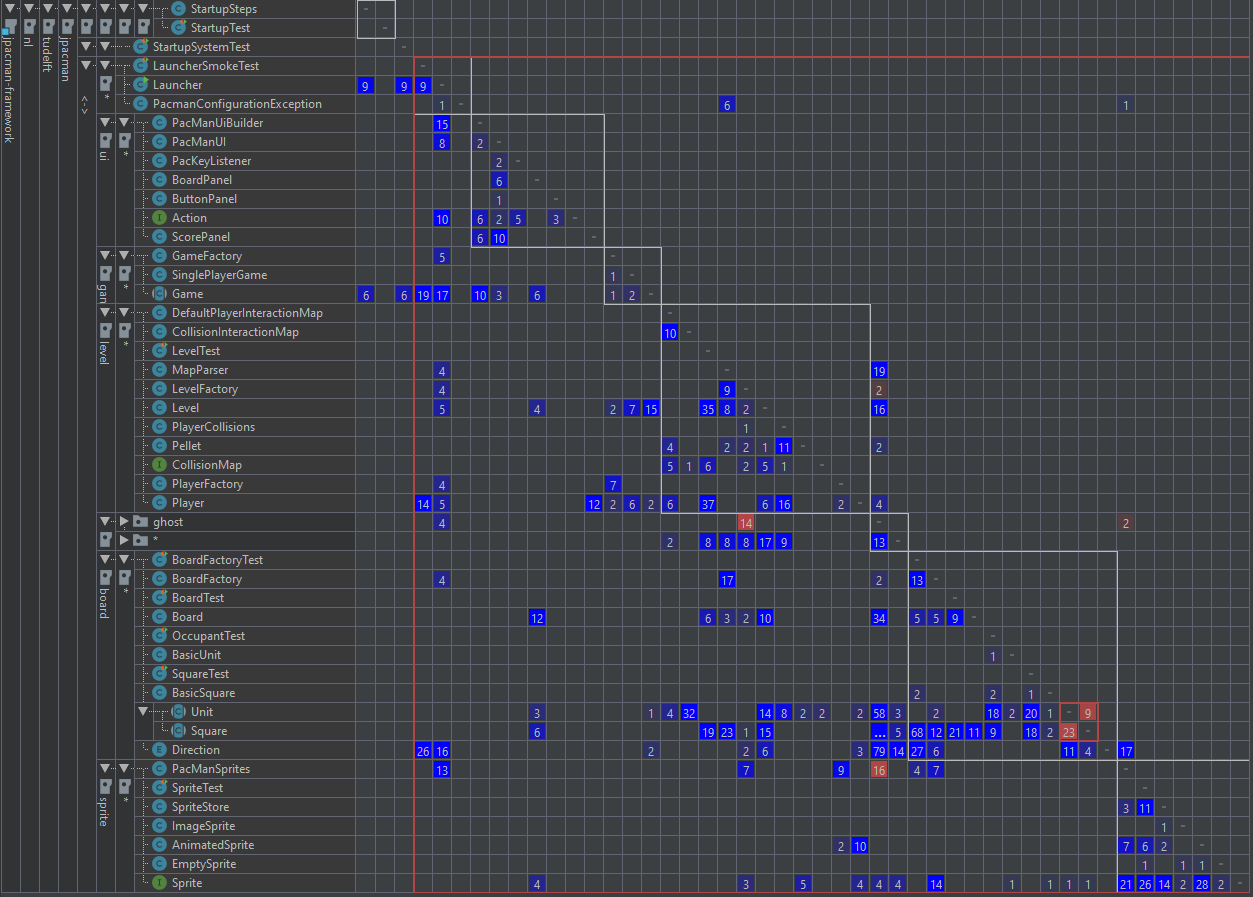
\includegraphics[width=\linewidth]{imgs/matrix dependencies.PNG}
    \caption{Matrix of Dependencies}
    \label{fig:DependenciesMatrixS1}
\end{figure}

\paragraph{Javadoc Coverage (MetricsReloaded)}

With the plugin \textit{MetricsReloaded} of \textit{IntelliJ}, we can assess few metrics like the Javadoc coverage (see Figure ~\ref{tab:javadocCoverageS1}). We observe that the project is fairly covered by the javadoc.

\begin{table}
    \centering
    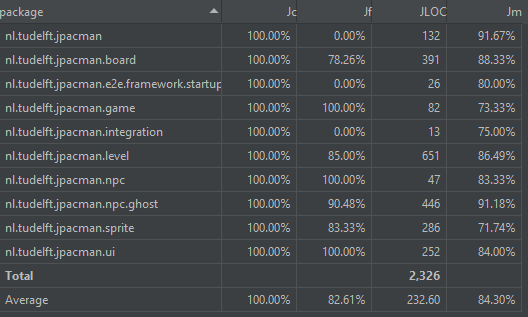
\includegraphics[width=\linewidth]{imgs/JavaDocCoverageS1.PNG}
    \caption{Coverage of the javadoc for the system 1}
    \label{tab:javadocCoverageS1}
\end{table}

\subsubsection{Dynamic Analysis}

\paragraph{Running tests \& Test Coverage (IntelliJ Build-Run)}

By running the tests provided with the project, 45 of 45 tests passed. Furthermore, IntelliJ provides a tool to assess the coverage of tests (see Table ~\ref{tab:TestCoverageS1}). Looking at the \textit{Method, \%} column, it's fairly well covered. We see that the Package \textit{level} is covered at 66\%. \\

In the Table ~\ref{tab:TestCoverage2S1}, we get more detailed information and observe that two classes are not tested, \textit{CollisionInteractionMap} and \textit{DefaultPlayerInteractionmap}. Furthermore, another class, \textit{LevelFactory} is covered at 50\%. Some enhancement can be done for it.

\begin{table}
    \centering
    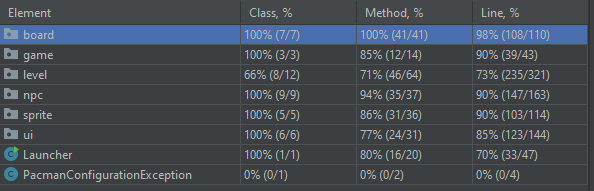
\includegraphics[width=\linewidth]{imgs/testCoverageS1.PNG}
    \caption{Test Coverage for the system 1}
    \label{tab:TestCoverageS1}
\end{table}

\begin{table}
    \centering
    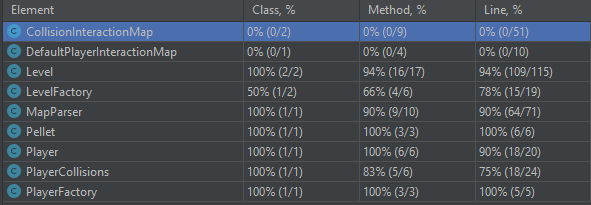
\includegraphics[width=\linewidth]{imgs/testCoverage2S1.PNG}
    \caption{Test Coverage Package level for the system 1}
    \label{tab:TestCoverage2S1}
\end{table}

\newpage
\subsection{System 2 (Rémy)}
\subsubsection{Generalities}

First of all, this is noticeable that authors provide some documents coupled with the implementation, even if it is not mentioned in the README file. This additional material is available under the \texttt{out/} directory at project roots and comprises :
\vspace{0.1cm}
\begin{itemize}
\item A \texttt{.pdf} file describing shortly the game, the controls and the multiplayer (2 players) mode available

\item A complete class diagram covering the whole implementation

\item A sequence diagram stating the execution flow when Pacman arrives on a cell and so ``eat" what is at this place

\item A graph of the mathematical function used to correlate difficulty with player's progression
\end{itemize}

We also observe that in this Pacman implementation maps are modelized under \texttt{.tmx} format, that is a popular way to deal with board games\footnote{\url{https://doc.mapeditor.org/en/stable/reference/support-for-tmx-maps/}}. Only one single basic map is provided\footnote{Actually the TMX file is never used, the map is rewritten in code as-is}.\\

The project structure is classic, we have \texttt{main} and \texttt{test} separation under the \texttt{src} directory, each containing packaged sources. The building system provided with the implementation is hold by Gradle. So a switch to Maven will be required to comply with directives.


\subsubsection{Static Analysis}

\paragraph{Code metrics (CodeMR)}

CodeMR allows to get an overall idea of the actual health of the system considering several metrics. The dashboard illustrated by \wordlink{Figure}{fig:S2_codeMR_dashboard} informs this software is doing quite good.

\begin{figure}[h]
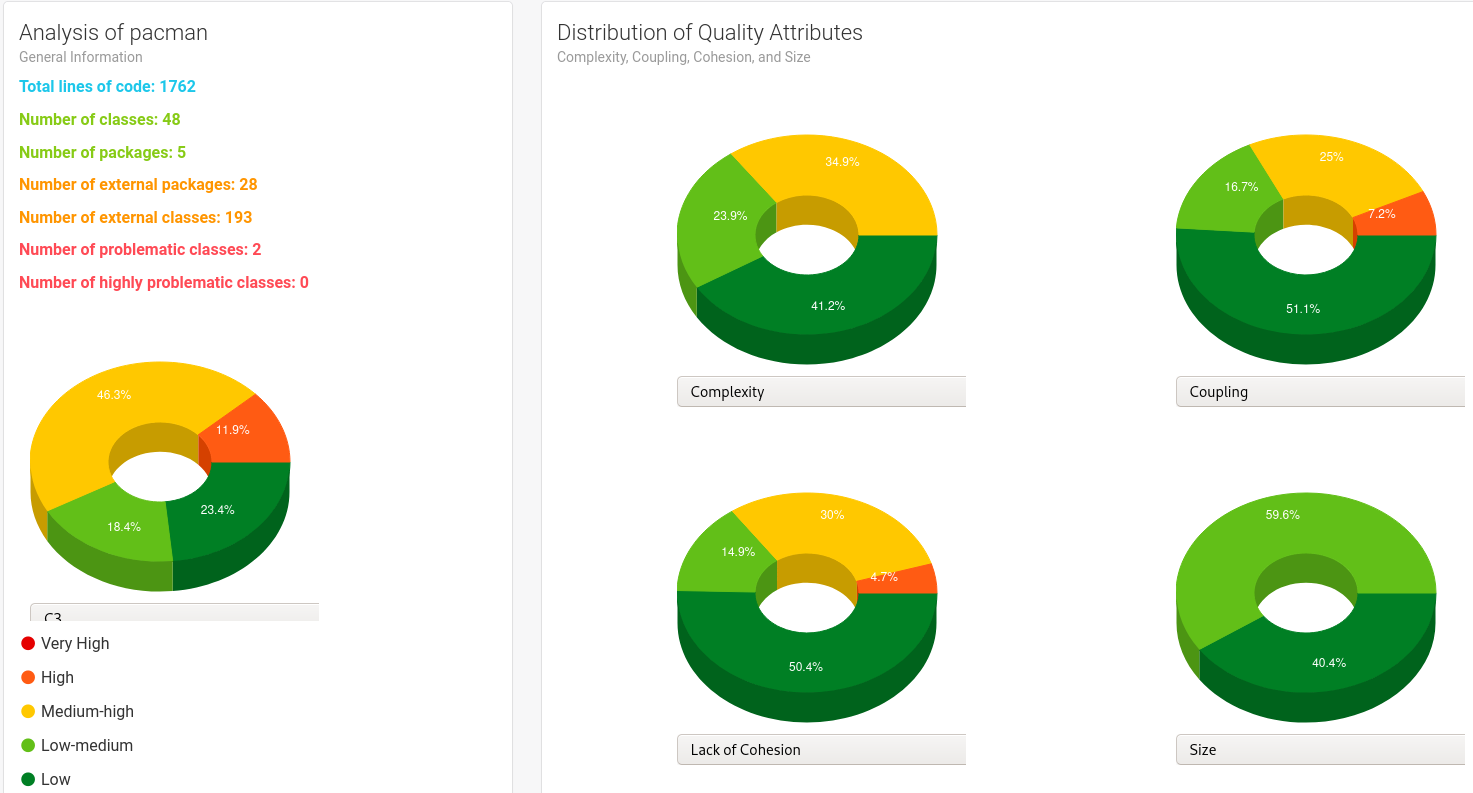
\includegraphics[width=\linewidth]{S2-codeMR_dashboard}
\caption{CodeMR dashboard summarizing health of system 2}
\label{fig:S2_codeMR_dashboard}
\end{figure}

\newpage

The \wordlink{Figure}{fig:S2_codeMR_packages} illustrates also the C3 metric but coupled with detailed packages view. We notice authors apparently tried to follow some Model-View-Controller pattern to design their application. The C3 metric is defined as the maximum between 3 other well representative metrics : \textit{Coupling}, \textit{Cohesion} and \textit{Complexity}. These are defined in the codeMR documentation\footnote{\url{https://www.codemr.co.uk/documents}}. We notice that, following the dashboard overview, two classes are impacting the software quality from the point of view of C3 metric.
\vspace{0.2cm}
\begin{figure}[h]
\centering
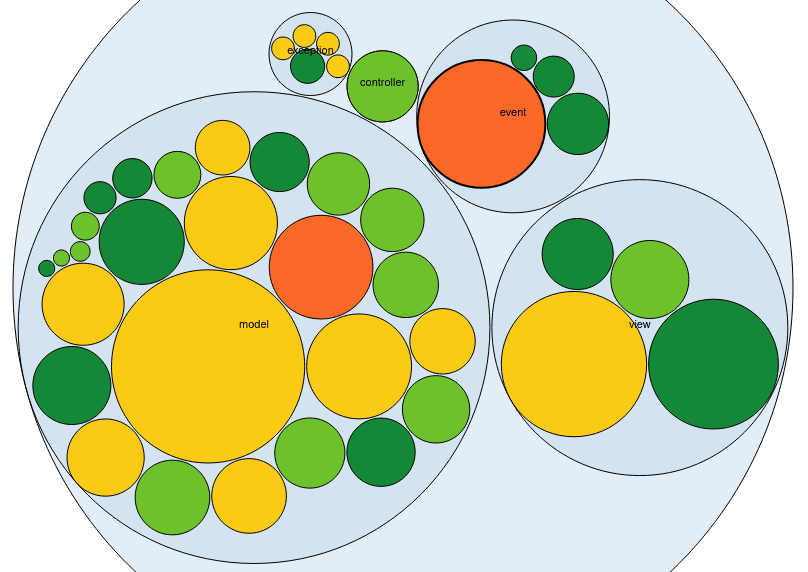
\includegraphics[width=0.8\linewidth]{S2-codeMR_packages}
\caption{C3 Metric by package for system 2}
\label{fig:S2_codeMR_packages}
\end{figure}

The details of the measurements on the two more problematic classes are given by \wordlink{Figure}{fig:S2_workerProcess} and \wordlink{Figure}{fig:S2_ghost}, for respectively \textit{event.WorkerProcess} and \textit{model.Ghost}. For both, two metrics are considered as high value, the meaning described by CodeMR is
\begin{itemize}
\item LTCC : The Lack of Tight Class Cohesion metric measures the lack cohesion between the public methods of a class. That is the relative number of directly connected public methods in the class. Classes having a high lack of cohesion indicate errors in the design.
\item LCOM : Measure how methods of a class are related to each other. Low cohesion means that the class implements more than one responsibility. A change request by either a bug or a new feature, on one of these responsibilities will result change of that class. Lack of cohesion also influences understandability and implies classes should probably be split into two or more subclasses.
\end{itemize}

In addition, for \textit{event.WorkerProcess} we have :
\begin{itemize}
\item CBO : The number of classes that a class is coupled to. It is calculated by counting other classes whose attributes or methods are used by a class, plus those that use the attributes or methods of the given class.
\item AFTD : Access to Foreign Data is the number of classes whose attributes are directly or indirectly reachable from the investiggated class. Classes with a high ATFD value rely strongly on data of other classes and that can be the sign of the God Class.
\end{itemize}

Other codeMR metrics did not revelate relevant problems in the implementation.

\newpage

\begin{figure}[h]
\centering
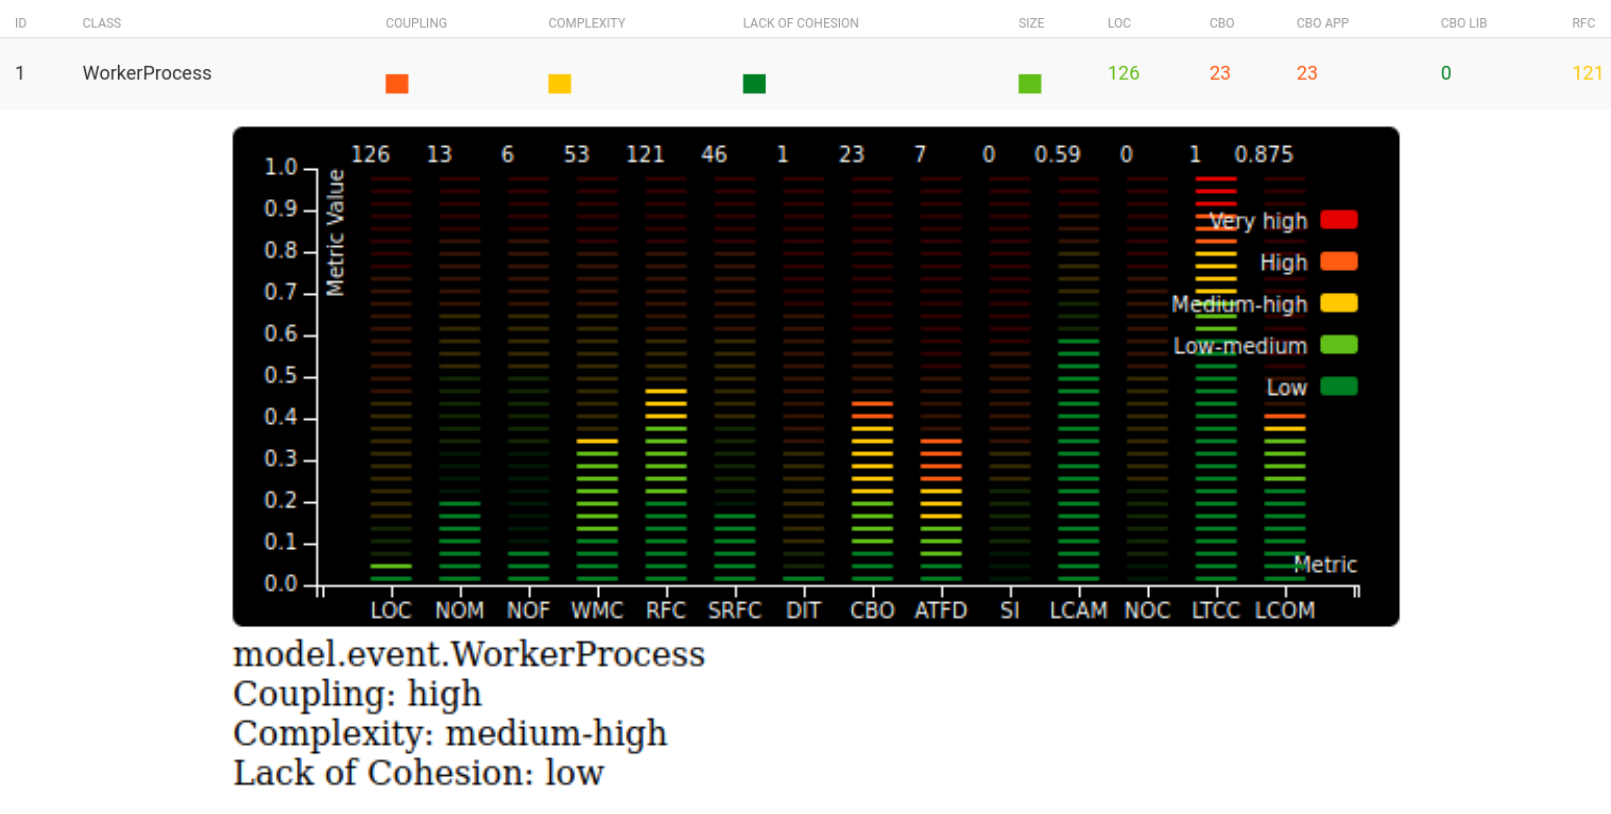
\includegraphics[width=0.9\linewidth]{S2-WorkerProcess_full}
\caption{\textit{event.WorkerProcess} class main metrics measurements}
\label{fig:S2_workerProcess}
\end{figure}

\begin{figure}[h]
\centering
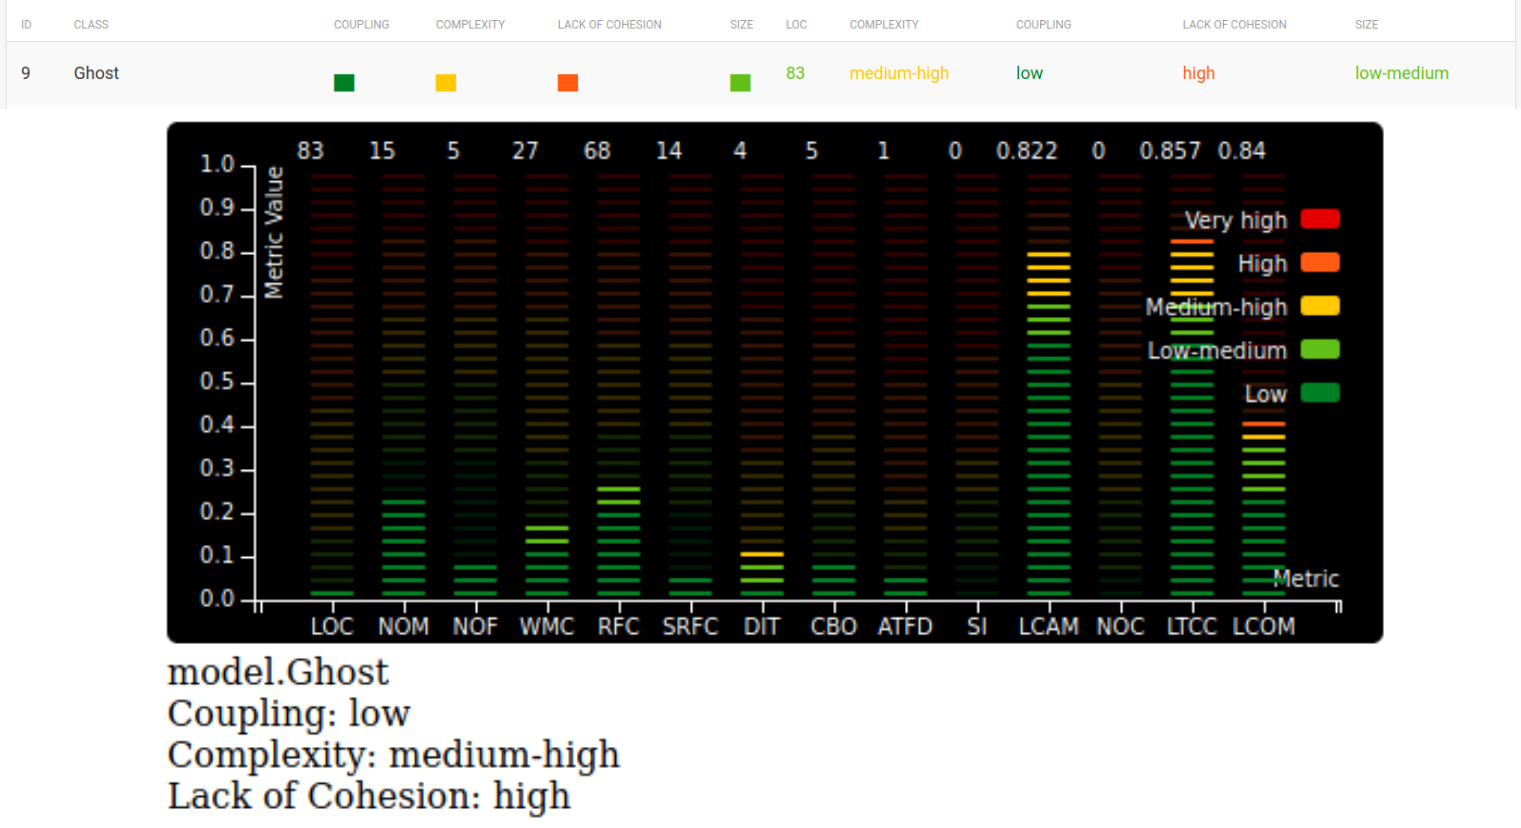
\includegraphics[width=0.82\linewidth]{S2-Ghost_full}
\caption{\textit{model.Ghost} class main metrics measurements}
\label{fig:S2_ghost}
\end{figure}
  
\newpage

\paragraph{Dependencies (CodeMR, Intellij analyzer)}

CodeMR allows also to inspect dependency relations between classes coupled with the metrics measured for each. We observe in the \wordlink{Figure}{fig:S2_inheritance} the same structure that in the class diagram. Once again the class \textit{event.WorkerProcess} is displayed as problematic, being too complex and coupled with other classes.\\

We use the standard built-in tool of IntellIJ IDEA to instantiate the dependency matrix, illustrated by \wordlink{Figure}{fig:S2_dep_matrix}. We clearly see reading 8th column that \textit{event.WorkerProcess} depends on a lot of other classes from package \textit{model}. This is also the case for \textit{model.Map} that presents a lot of cyclic dependencies (red marked).

\paragraph{Compliance \& bad smells (PMD, Designite)}

PMD is a statical analyzer that checks for problems of several natures in the code. It detected more than 1500 violations in the system 2, related to various topics (see \wordlink{Figure}{fig:S2_PMD}).

\vspace{0.3cm}

\begin{figure}[h]
\centering
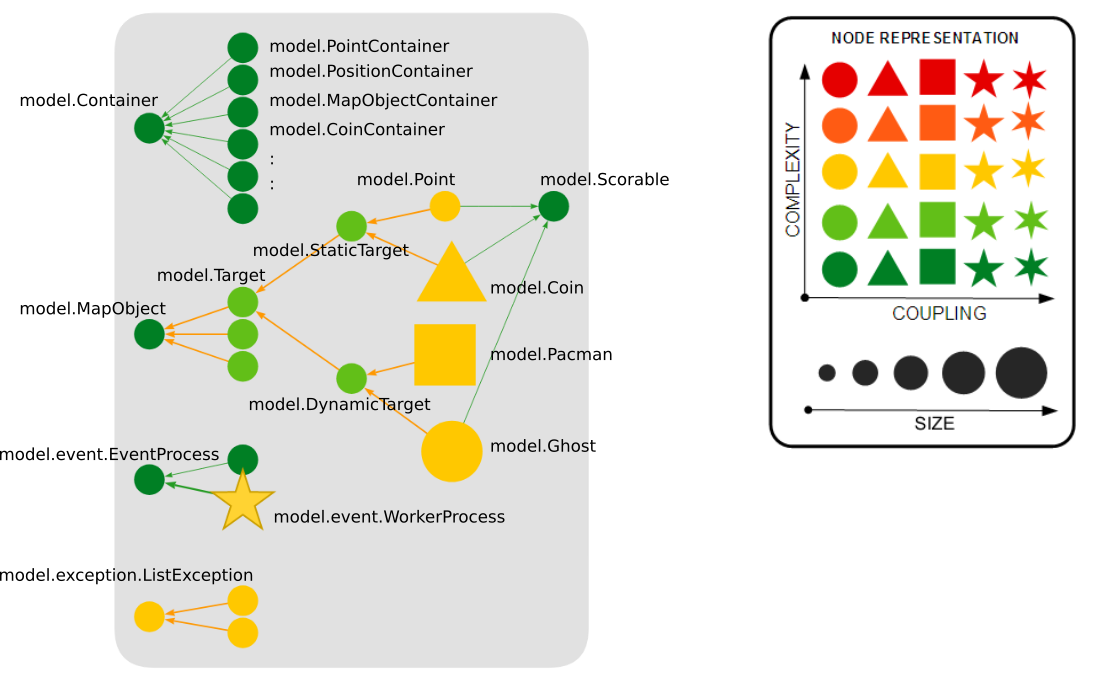
\includegraphics[width=0.8\linewidth]{S2-named_inheritance}
\caption{Inheritance relations between classes in system 2}
\label{fig:S2_inheritance}
\end{figure}

\vspace{0.4cm}

\begin{figure}[h]
\centering
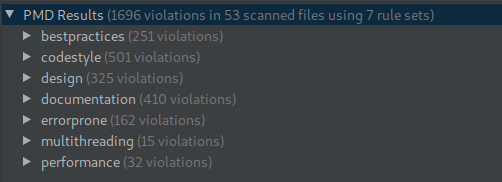
\includegraphics[width=0.7\linewidth]{S2-PMD_results}
\caption{Violations found by PMD in system 2}
\label{fig:S2_PMD}
\end{figure}

\newpage

\begin{figure}[h]
\centering
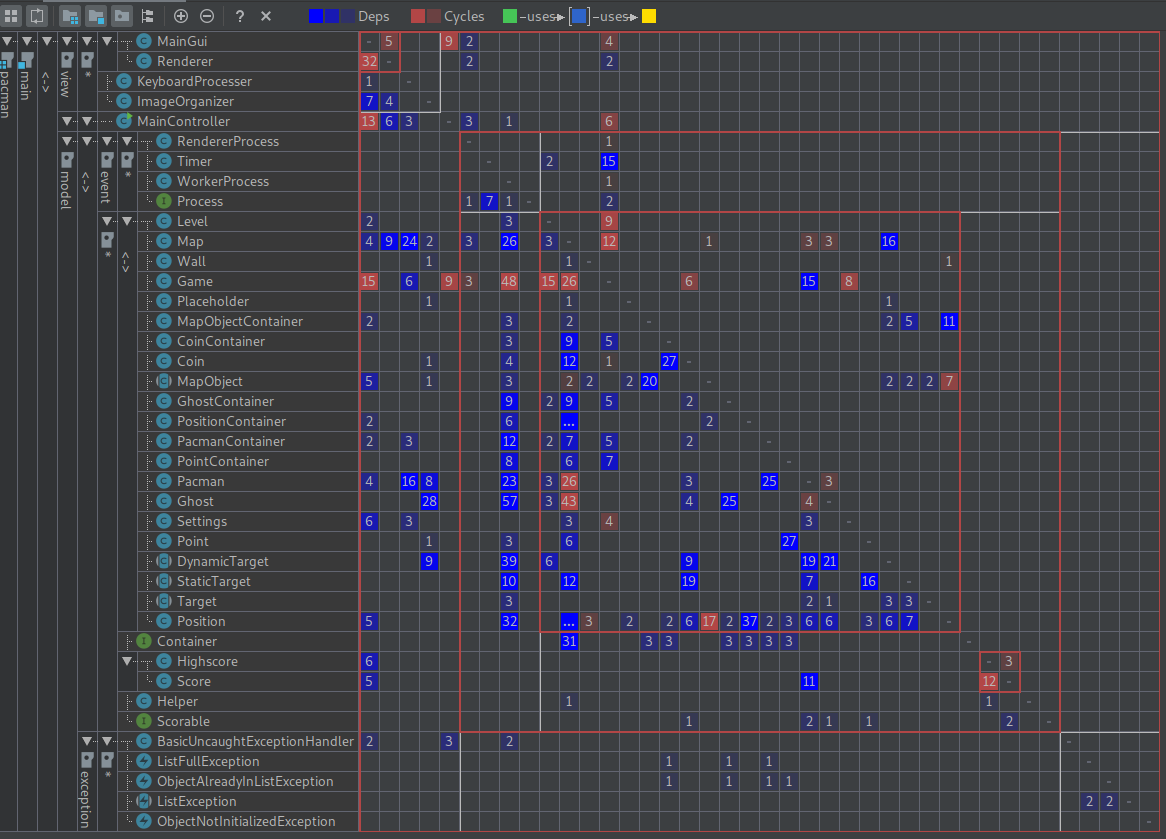
\includegraphics[width=0.9\linewidth]{S2-dep_matrix}
\caption{Dependency matrix for system 2}
\label{fig:S2_dep_matrix}
\end{figure}

\vspace{0.1cm}

\newpage

Designite is used to detect bad smells, a summary of the analyse is presented by \wordlink{Figure}{fig:S2_designite}. The number of lines of code and classes is higher than the ones returned by CodeMR because the test sources were considered in the analysis.

\begin{figure}[h]
\centering
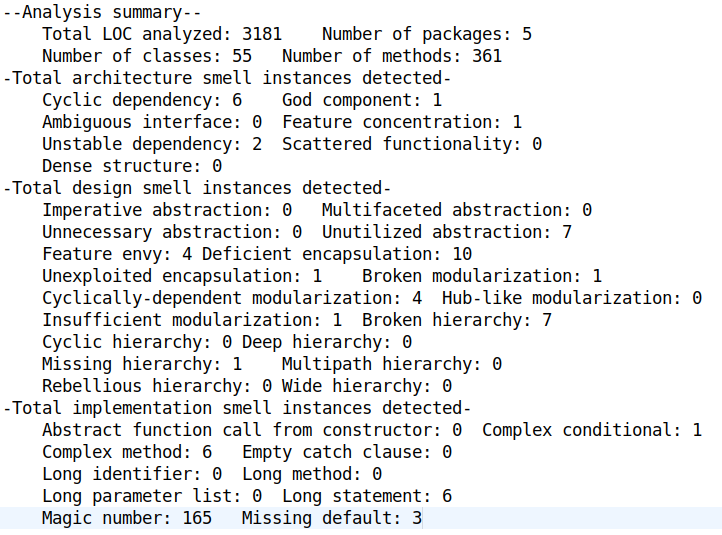
\includegraphics[width=0.65\linewidth]{S2-designite}
\caption{Designite in-line use results for system 2}
\label{fig:S2_designite}
\end{figure}


\paragraph{Javadoc coverage (MetricsReloaded)}

We use the IntellIJ MetricsReloaded plugin and its metric "Javadoc coverage" to get an overview of how complete is the initial javadoc. As shown by \wordlink{Figure}{fig:S2_javadoc}, this is the case.

\vspace{0.2cm}

\begin{figure}[h]
\centering
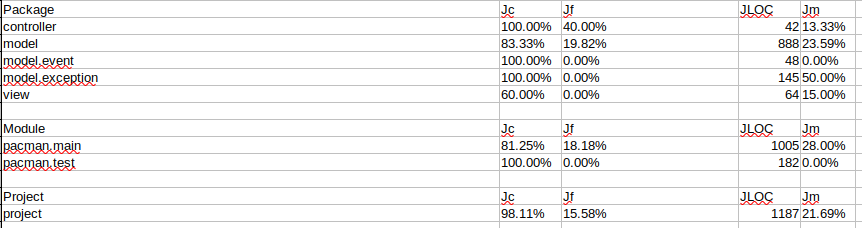
\includegraphics[width=0.75\linewidth]{S2-javadoc}
\caption{Javadoc coverage for system 2}
\label{fig:S2_javadoc}
\end{figure}

\newpage

\subsubsection{Dynamic Analysis}

\paragraph{Running tests}

Among the already written tests, 3 out of 67 failed at running time. The three tests are in \textit{model.LevelTest} (\textit{testGetLevel}, \textit{testSecondsForCoin} and \textit{testNextLevel}). 

\paragraph{Test coverage (Intellij built-in tool)}

IntellIJ provides run configurations to dynamically analyze what are the parts of source codes covered by launched tests. Considering whole test packages, summary of the results are given by \wordlink{Figure}{fig:S2_test_coverage}. We observe the implementation benefits of a good test coverage, the most laking part is package \textit{view} but it makes sense by its nature.

\newpage

\begin{figure}[h]
\centering
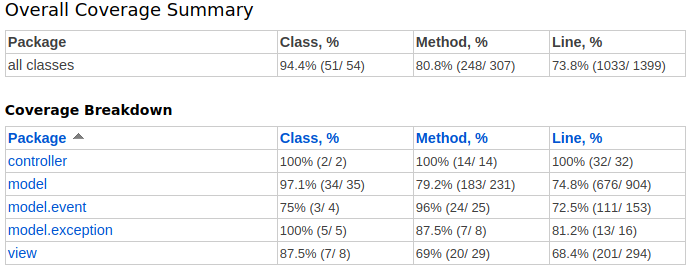
\includegraphics[width=0.75\linewidth]{S2-test_coverage}
\caption{Test coverage for system 2}
\label{fig:S2_test_coverage}
\end{figure}

\newpage

\subsection{System 3 (Robin)}
\subsubsection{Generalities}

For this project the author provides no documents.

The Pacman maps are modelized under a \texttt{.txt} format, where each type of case are attributed a certain letter. 

We also observe that in this Pacman implementation maps are modelized under \texttt{.tmx} format, that is a popular way to deal with board games\footnote{\url{https://doc.mapeditor.org/en/stable/reference/support-for-tmx-maps/}}. Only one single basic map is provided.\\


In the project structure, there is \texttt{test} and \texttt{src} directory. In the first one there are the test classes and in the latter there are two directories, \texttt{Ressources} and \texttt{pacman\_infd}. In \texttt{Ressources} we have the Pacman maps that are modelled under a \texttt{.txt} format, where each type of case are attributed a certain letter, and also the sound files in \texttt{.wav} format. \texttt{pacman\_infd} contains all Java classes.
\\

The building system provided with the implementation is hold by Ant. So a switch to Maven will be required to comply with directives.


\subsubsection{Static Analysis}

\paragraph{Code metrics (CodeMR)}

 The dashboard illustrated by \wordlink{Figure}{fig:S3_codeMR_dashboard} informs this software is doing really good.

\begin{figure}[h]
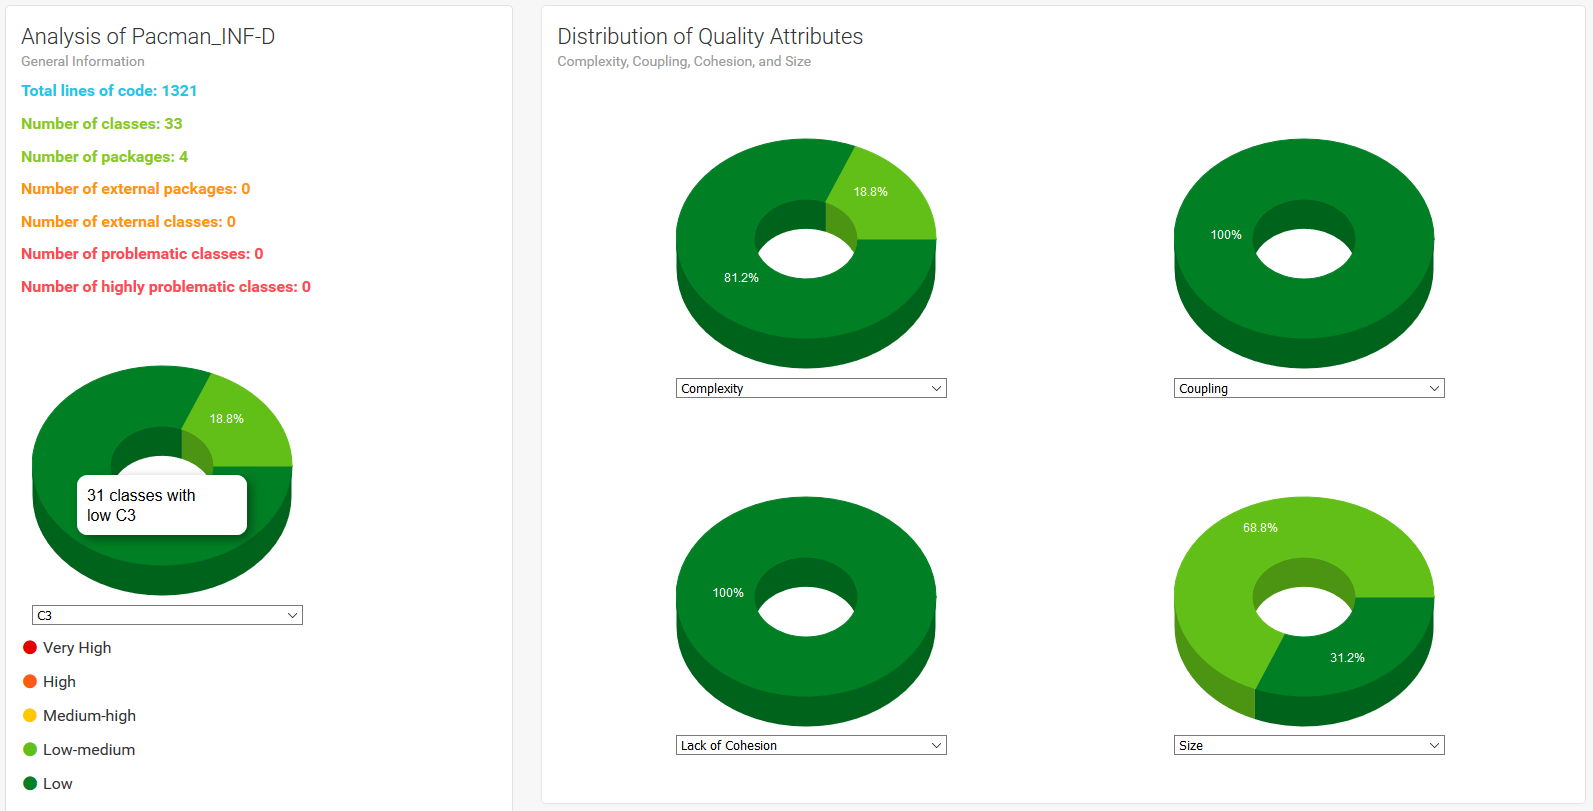
\includegraphics[width=\linewidth]{S3_codeMR_dashboard.png}
\caption{CodeMR dashboard summarizing health of system 3}
\label{fig:S3_codeMR_dashboard}
\end{figure}

\newpage

The \wordlink{Figure}{fig:S3_codeMR_packages} illustrates also the C3 metric but coupled with detailed packages view. We can see that every classes is doing good. 
\vspace{0.2cm}
\begin{figure}[h]
\centering
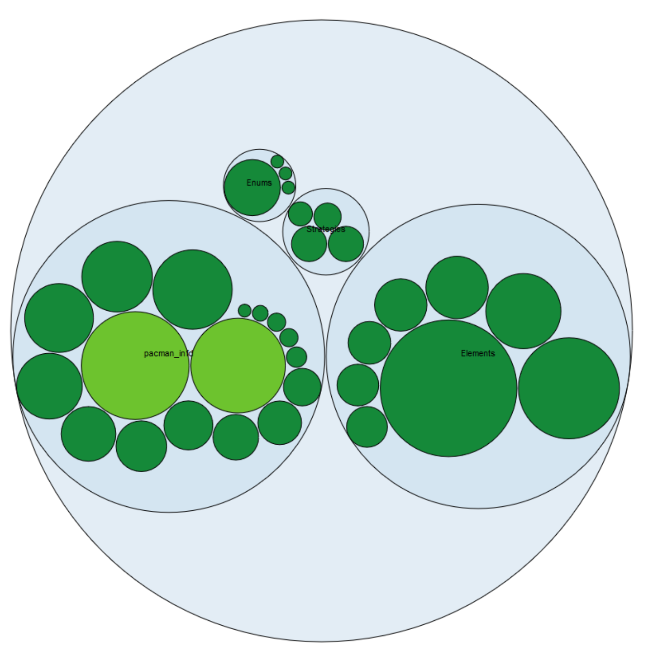
\includegraphics[width=0.8\linewidth]{S3_codeMR_packages.png}
\caption{C3 Metric by package for system 3}
\label{fig:S3_codeMR_packages}
\end{figure}

There are no problems in the classes for almost all the metrics, only for two of them, we can see a problem: the Lack of Tight Class Cohesion  and the lack of Cohesion of Methods. 
For the first one, nine classes have High or Very-High risks like the GameController or the View. And for the latter, three classes have High risks: GameController, ScorePanel and GameWorld.

  
\newpage

\paragraph{Dependencies (CodeMR, Intellij analyzer)}


We use the standard built-in tool of IntellIJ IDEA to analyze the dependency matrix, the result is shown on  \wordlink{Figure}{fig:S3_dep_matrix}. 


\begin{figure}[h!]
\centering
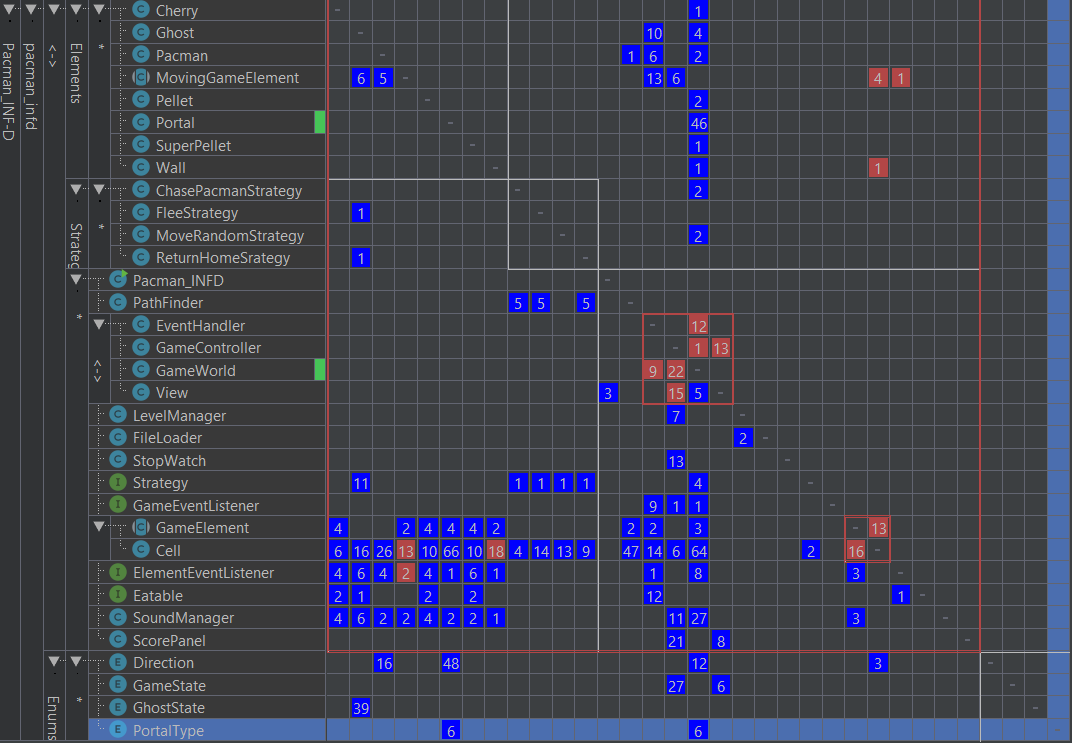
\includegraphics[width=0.8\linewidth]{dependencyM.png}
\caption{Dependency matrix for system 3}
\label{fig:S3_dep_matrix}
\end{figure}

\newpage

\paragraph{Compliance \& bad smells (PMD, Designite)}

We first used PMD, it detected more than 1343 violations in the system 3, here is the result:
\begin{itemize}
    \item 1343 violations: 
    \begin{itemize}
        \item best practice: 54
        \item code style: 414
         \begin{itemize}
            \item 125: method arg could be final 
            \item 98: local var could be final
            \item 60: short variable name
        \end{itemize}
        \item design: 503
        \begin{itemize}
            \item 449: most is law of demeter 'only talk to friends'  
            \item 31: immutable field: private field values never change once object init could be 			                   final
        \end{itemize}
        \item documentation: 192
        \item error prone: 167
        \begin{itemize}
            \item 70: Bean member should serialize: make variable transient or static
            \item 21: avoid literal in if condition
        \end{itemize}
        \item performance: 13
    \end{itemize}
\end{itemize}
		

 The result of Designite analysis is on \wordlink{Figure}{fig:S3_designite}. 

\begin{figure}[h]
\centering
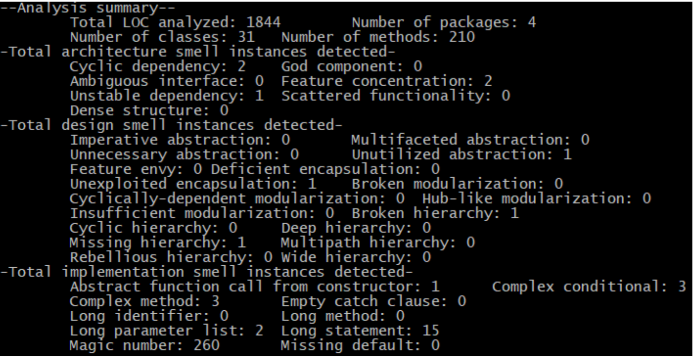
\includegraphics[width=0.85\linewidth]{S3-designite.png}
\caption{Designite in-line use results for system 3}
\label{fig:S3_designite}
\end{figure}


\newpage


\subsubsection{Dynamic Analysis}

\paragraph{Test coverage (Intellij built-in tool)}

The test coverage of the given tests was analyzed, and the three following figures \ref{fig:S3_test_coverage}, \ref{fig:S3_test_coverage0} and \ref{fig:S3_test_coverage2} give the results. We can see that only 28\% of the code is tested and 69\% of the classes. We can see that neither of the strategies in the Strategies packages is tested, and in the Elements package only 12 methods is tested on the 59 methods that are available.


\begin{figure}[h!]
\centering
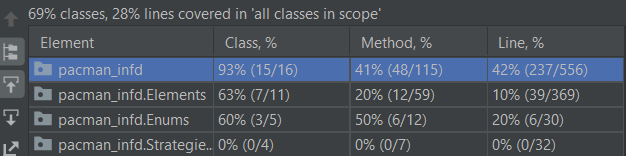
\includegraphics[width=0.75\linewidth]{testCov.png}
\caption{Test coverage for system 3}
\label{fig:S3_test_coverage}
\end{figure}

\begin{figure}[h!]
\centering
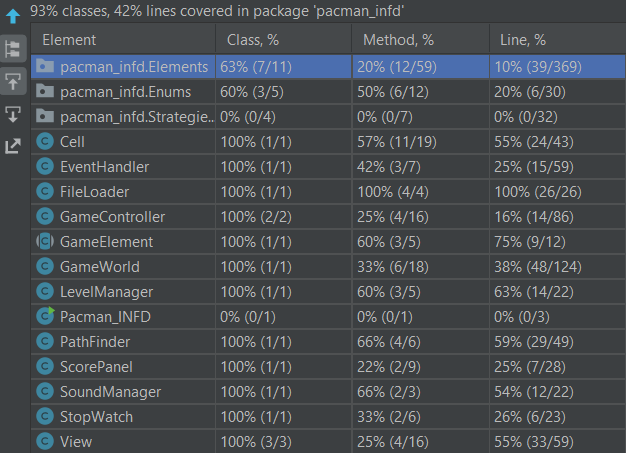
\includegraphics[width=0.75\linewidth]{testCov2.png}
\caption{Test coverage of the pacman\_infd package}
\label{fig:S3_test_coverage0}
\end{figure}

\begin{figure}[h!]
\centering
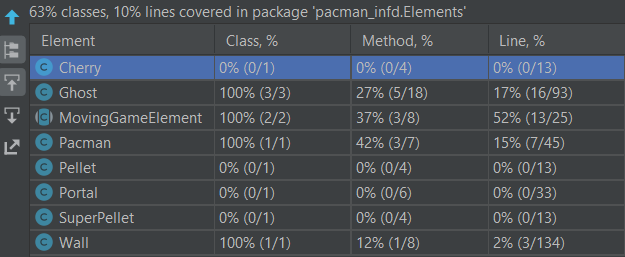
\includegraphics[width=0.75\linewidth]{testCov3.png}
\caption{Test coverage for the Elements package}
\label{fig:S3_test_coverage2}
\end{figure}

\newpage

\subsection{Comparaison of the 3 systems}

From what we discussed, it appears that the system 1 is definitively the best. It is already fully documented and well tested, so robust (for example using \texttt{assert} Java statement). Even if it doesn't appear clearly in the analysis, the structure and the patterns used are better as well. For example, system 2 overuses the Singleton design pattern, leading to a non structured code. This also leads to some bugs the authors apparently didn't correct.\\

The number of test doesn't make it all, as system 2 proves. There are a lot of tests, but some just don't pass or are empty. Even if apparently good using CodeMR, system presents some catastrophic classes like \texttt{Wall}, and some bad programming practice as very long \texttt{else-if} statements that gives an idea about how much authors don't apply well OOP programming guidelines. 

\newpage
\clearpage
\section{Quality improvement}
\subsection{System 1 (BOOSKO Sam)}

In general, the provided implementation didn't need improvement but few were done like making an object as a parameters for method with too many parameters. Furthermore, few magic numbers were fixed in unit test implementation. Mainly, magic numbers were in testing codes, then it's normal to have them there. It's more readable to understand them and write them.\\

The part of the implementation in \textit{MapParser} which manage the creation of element of the game from a text file were modify to increase the readability and help new developers to add new elements in the project. At first, it was done with a switch case on a \textit{Char}. To make it more modular, an Interface, called \textit{ISquareBuilder}, was create. This class take as parameter and object, \textit{AddSquareParameters}, which contains all information of the game to create easily and new element. An abstract class, \textit{ADefaultSquareBuilder}, implementing this interface, is also created. This abstract class helps to reduce the duplication code. Finally, it's pretty easy to add a new element on the grid by adding the \textit{Char} key and the responding ISquareBuilder. \\
\newpage

\subsection{System 2 (Rémy)}

We employ the following methodology to improve the system in its current state :
\begin{enumerate}
\item Reviewing the whole code and correct problems of form. It allows to acquire a global overview of the implementation to lead next steps and improve code quality on a per-class basis. These refractorings comprise, among others :
\begin{itemize}
\item completing the Javadoc
\item getting rid of forgot/useless artifacts
\item detecting and correcting code smells
\end{itemize}
The main tool used during this step will be the IDE (IntellIJ) and plugins associated with like Designite, which allow on-the-fly analysis and pointing out problems in the code itself.


\item Reviewing the system structure and correct structural design problems. From the acquired global overview, it is possible to have an idea of drawbacks implied by the system design. The refractoring will occurr at a class-to-class relations level, and will then impact package structure level. Some tools and metrics, for example from CodeMR, can be used to leas this step : a class reported too long may be splitted into more than 1 class, inheritance should be used better, etc.

\item If some tests are not passing, find the reason and correct them.

\item Complete the tests based on test coverage reports generated (from IntellIJ).
 
\end{enumerate}
\vspace{0.2cm}
Of course, after each of these steps, the current yet written tests must be launched to control the consistence of the implementation.

\subsubsection{Step 1}

\indent\par We read through the whole code and corrected what had to be in a first time. Some smells are straightforward, like avoiding Magic Numbers detected by Designite. The help of IntellIJ is precious to get rid of some deprecated/forgot code artifacts the authors left. Some problems reported by Designite are not regarding the actual usage and left as-is.

\subsubsection{Step 2}

\indent\par It was figured out the current implementation presents some drawbacks. It is mainly related to code duplication for already written objects for \texttt{Container} purposes (can be found in provided class diagram). The fact is that authors wanted to write an overlayer to describe different collections of other objects in the implementation (\texttt{Coin} (= pills), \texttt{Point}, etc.). But they wrote a specific class for every type of object to contain, albeit implementing the common \texttt{Container} interface, this design is very poor and ineleguant, leading to code duplication and increased number of classes. Keeping in mind what were each class written for, we redisigned this part of the implementation in a better way. It also brought the occasion to cluster \texttt{Container} class concerned in a new package to improve the project structure readability.\\

The resulting structure is depicted by \wordlink{Figure}{fig:S2_containers}. We now consider to pass through a \texttt{Containers} class to construct any \texttt{Container} needed in the rest of the implementation. Its static methods instantiate the right container with adapted type of content from generic classes. These instances are shown in orange in the \wordlink{Figure}{fig:S2_containers}. The restricted typing \texttt{E extends MapObject} allows getting element(s) considering a \texttt{Position} object. A \texttt{PositionContainer} is a specialized container to hold coordinates (already present in original code), so we dont use an index but form a key from the couple ($x$, $y$). The method \texttt{getRange(..)} allows to get a subset of contained positions, considering a rectangle selection formed from two positions given in parameters. For some object types (\texttt{Point}), an overload is necessary to comply with the rest of the implementation. Anyway, this is somehow masked because all containers instances are retrieved from the class \texttt{Containers} mentioned above,  not represented in the figure.

\newpage

\begin{figure}[h]
\centering
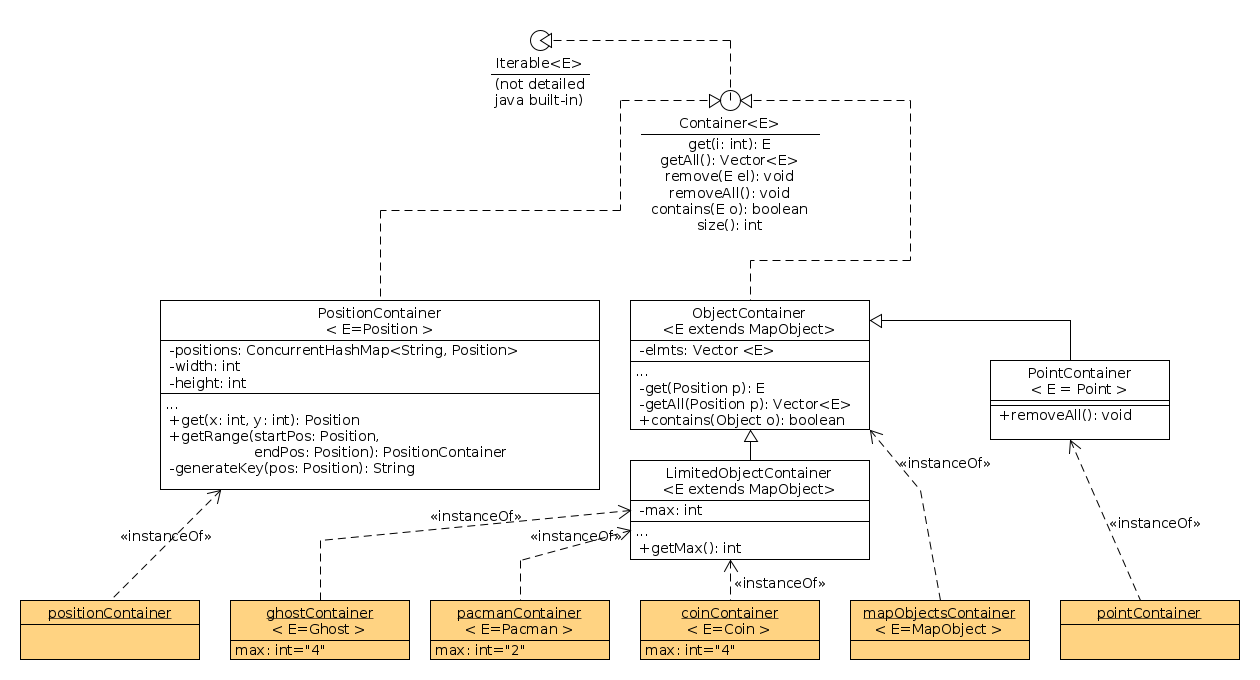
\includegraphics[width=\linewidth]{S2-classdiagram_containers}
\caption{New class structure for \texttt{Container}s part of the implementation}
\label{fig:S2_containers}
\end{figure}


An other problem is related to the \texttt{Map} class. We observe the Map itself and the objects that will represent it in the application are instantiated in raw. Coordinates for each element are given in the code itself, that is a bad practice. However, due to the lack of time and considering the picked extension doesn't relate to maps, a trade-off is taken. A new class \texttt{MapPlacer} is written to hold the placement of \texttt{MapObjects} on the declared possible \texttt{Positions} of the unique considered map. It cleans up the code of the original class \texttt{Map} that should only hold dynamic operations such as reinitializing the content of the map when the player passes a level.\\

Concerning package structure, some changements were also needed because the \texttt{model} package had no sub-level (grouping almost 30 classes). We added a subpackage \texttt{model.container} that holds all the hierarchy depicted above and another \texttt{model.mapobject} to group all classes standing for the actors/components of the game (\texttt{Wall}, \texttt{Pacman}, \texttt{Coin}, etc.).

\subsubsection{Step 3}

\indent Some already written tests were not passing, or passing but throwing an exception. That was mainly due to the management of multithreading and game reseting not properly. Also, the usage of \texttt{static} elements lead to inconsistencies. Leveraging some adjustements in the source code, we managed to get the system more consistent and the tests passing in a determenistic behaviour.

\subsubsection{Step 4}

\indent \par The provided existing tests are numerous but not relevant for some. Firstly, there are empty tests, whose only signature is written. They were filled in the right way to evaluate what they're expected to. Some others focus only on get/accessors and methods that are even never used in the rest of the implementation. So, tests oriented to behavior evaluation are mainly missing. We added some for \texttt{Map}, \texttt{Ghost}, \texttt{Pacman}, etc. They aim to ensure the game is running as expected. More diverse additions were done all over to improving testing quality.\\

As some new classes have been written to improve the system quality, the associated tests were also written. We have \texttt{PositionContainerTest} and \texttt{TimerTest} to evaluate the new implementation parts described above.

\newpage
\subsection{System 3 (Robin)}

The first change was changing the building system from Ant to Maven. 
\\

After that, we used PMD and Designite to find problems and refactor them. The access of classes, methods and variables was changed depending of the need, it was set to protected or private if it was possible. Some variables were set to final. We found magic number, and tried to remove them if it was posisble and usefull. 
\\

Then some long methods were divided into multiple methods for more readability. Some switch-case were also added instead of long if-else. Some new method were also added.
\\

The Direction Enumerator class was changed to make it smaller and not just a succesion of switch-case. 
\\

The structure of the classes was also changed. The source code of the project is now divided in 5 packages: Elements, Enums, Fileloader, Game and Strategies. Elements contains all the moving elements of the game, like Pacman or the ghosts, and the other game elements like the cherry or the pellet. The Enums packages contains all the enumeration that are used in the project. The FileLoader package contains all the classes that are used to manage the loading of a level. Strategies contains all the strategies and pathfinders that are used by the ghosts. And the Game package contains everything else that is used for the game, the GameWorld, the Controller or the Listener for exemple.
\\

Then the GUI was changed for Pacman, before changing the code Pacman wasn't changing his orientation on the application, now we can see Pacman change it's orientation. There is also a little animation for the mouth of Pacman, he opens and shut his mouth to simulate eating. 
\\

Some new test where also created on the test package to cover more code. The different strategies of the Strategy package was tested. New tests fot the eating of pellet, cherry and super pellet was also created.
\\




\newpage
\section{Adding basic functionalities}
\subsection{System 1 (BOOSKO Sam)}

The provided project missed basic functionalities, such as the continuous PacMan Moving, fruit elements, power pellet...\\

The first feature added is the continuous PacMan moving, a new class is created for ot, \textit{PlayerController}. This class contains information from the game and have a scheduled action. This action is simply to move the pacman to the register position. This direction can be changed by a key listener. The speed of the pacman is managed here with two attributes, 1) $Speed$ and 2) $SpeedModifier$. With them, the final speed is compute as $speed * speedModifier$. Where the speed unit is the number of tiles per second. The speed modifier is thought to help the implementation of extensions.\\

Secondly, to be able to add new elements that pacman can eat on the board, the class \textit{Pellet} is edited to add an action \textit{onEat(Level level, Player player)} where the player is the pacman who ate the element. This action is called when a player have a collision with a pellet element. With this method, it was easy to implement the feature of scared ghosts (Pacman can eat a scared ghost) and the feature of new life by eating fruits.\\

Everything was thought to help another person to add new features from the sectioned extension. Adding a new element on the board take $1$ minute. The longest time being the implementation of the action performed of this new element.\\
\newpage
\subsection{System 2(Rémy)}

The following functionnalities were pointed out as missing in this system :

\begin{itemize}
\item The last two pills eaten in a Level must give an invicibility of 5 seconds instead of 7 seconds
\item A ghost must disappear when munched and respawn in the ghost base after 5 seconds
\item Consecutive eaten ghosts must give more points (200-400-800-1600)
\item There is a timer ruling each level (stoped when pacman is hunting)
\end{itemize}

\vspace{0.2cm}

The commit corresponding to the final version of the basic game is \\

\url{https://github.com/RemDec/pacman-system2/commit/cb5e36143d6ab84a9c02d80cd4c58ae56ff0e8aa}

 ~\\

These functionnalities are somehow straightforward to implement in this system. Of course some unit tests are written to verify the new behaviors. The only remark would go to the timer. As this system is intended to strengthen the difficulty increasing the ``refresh rate", this rate govern the display frequence. This is why the displayed timer increments step-by-step (we avoid using new display threads to keep consistency and good integration in the actual system). As this timer feature was not present, new classes \texttt{Timer} and \texttt{TimerProcess} were written to be easily integrated with the already existing \texttt{Scheduler} (renamed, previously \texttt{Timer}). The timer has been integrated to the interface as depicted by \wordlink{Figure}{fig:S2_timer}.\\

It was also necessary to correct some hidden bugs related to the behavior of ghosts. Sometime when eaten, they stay at their position instead of respawning in their base. The code was modified to obtain the right behavior and some tests were added to ensure this. \\


\begin{figure}[h]
\centering
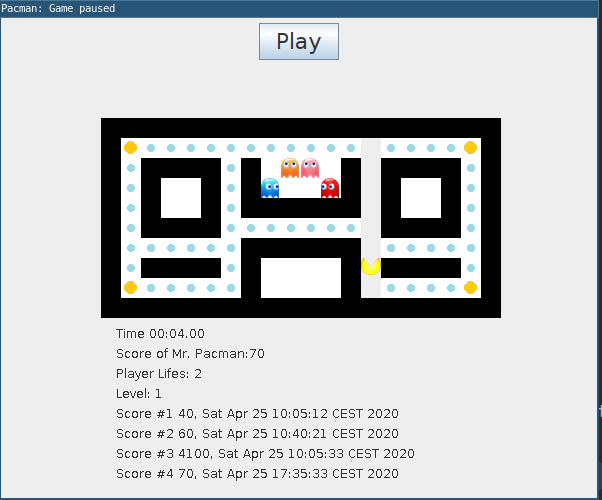
\includegraphics[width=0.6\linewidth]{S2-screen_timer}
\caption{New timer integrated in the interface (below the map)}
\label{fig:S2_timer}
\end{figure}

\newpage

\subsection{System 3 (Robin)}

\indent\par In this implementation, we couldn't advance to the next level once we finished eating all the pellets.  We first changed that. Now a level can be succeeded and when it's done we advance to the next level, there is 3 level in total but the first 2 are the same.
\\

The levels were also re-writen, in the levels there were some disconnected regions, so we removed that. 
\\

After that the behavior for the super pellet/power pill was also changed. The clock was not set in pause when the pill was activated. The score gained by eating the ghosts was also not the one set in the rules, so it was also changed. The time for the pills was also changed, the first two lasts 7 seconds and the last two lasts 5 seconds.
\\

Eating a cherry on the initial implementation wasn't making pacman gain an additional live, so that was also added. \\

The final commit,for the implementations can be found here :\\~\\
\url{https://github.com/irikay/pacman-system3/commit/c34569f5095c552876e3a12a91c8d73975448cbe}


\newpage
\section{Adding new features}
\subsection{System 1 (Rémy)}

\subsubsection{New features discussion}

\indent\par The integration of special fruits/boxes in this system is quite facilitated by the quality of the implementation, which allows to define new unities and their collision map in a generic way. It is done by subclassing \texttt{Unity} class or one of its already existing subclasses. For example, for new fruits that apply an effect within a given duration, a generic class \texttt{SpecialPellet} is written, extending \texttt{Pellet}. It handles the duration and resetting original state once exhausted. Each fruit is a short subclass of it (\texttt{PotatoPellet} for example) which implements its logic depending the associated effect. We managed to give a variation in each effect that makes sense with the current game state. For \texttt{PotatoPellet}, the more pacman has score, the juicier he looks for ghost so they are buffered for an increased duration. Note that we made the choice that duration effects are not cumulutative to keep the game clear and the current Pacman state always indicated to the player (thanks to the Pacman's skin). Though Pacman can still become a hunter during a special effect (indicated by ghosts skin).\\

Implementing special boxes is also somehow straightforward : we sublcassed \texttt{Unity} with \texttt{SpecialBox} and each box is a subclass of the latter. These boxes have an impact on the game logic and are not especially coupled with a duration. It lead to modifications on the collisions logic. For instance, \texttt{BridgeBox} implements bridges that required an introduction of the vertical level notion (\texttt{DOWN} and \texttt{UP}), a state associated with each unit. We reconsidered collisions to be handled occurring only between units in the same vertical level.\\

The detail about each special unit and the way effects vary depending current game state can be found in the corresponding class documentation. An illustration of the implemented special units is provided by \wordlink{Figure}{fig:S1_special} (illustrating actual effect is quite difficult for most, it should be played instead).\\


\begin{figure}[h]
\centering
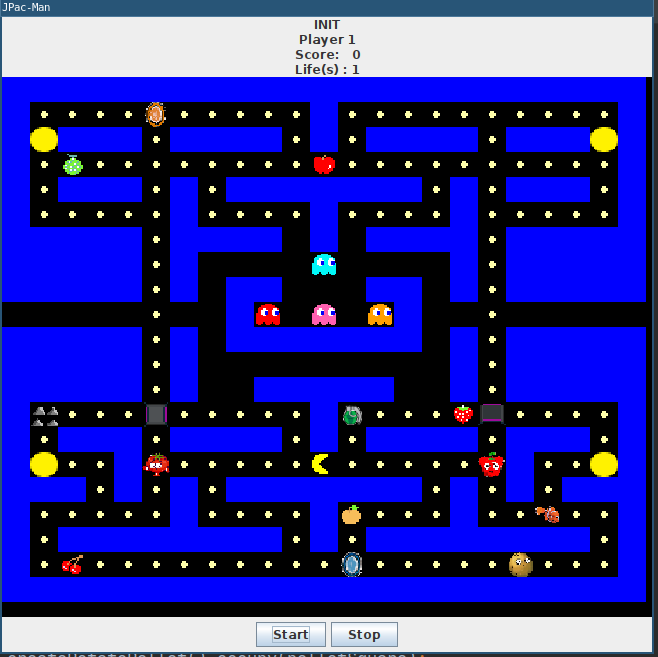
\includegraphics[width=0.62\linewidth]{S2-extension}
\caption{Illustrating all special units on the bottom of the map}
\label{fig:S1_special}
\end{figure}

\newpage

Apart from the effect of special units, it was also asked to make them dynamically spawn taking account the current state of the level. This new mechanic is handled by the class \texttt{SpecialUnitySpawner}. At a fixed time interval (7 seconds), a try is done to spawn a special unit on the board : this decision is made in a probabilistic fashion. The process accounts for the following guidelines :
\begin{itemize}
\item if the board is nearly empty (ie. there are a few pellets compared to the number initially present), it could be good to fill it a bit to change the destiny of this game that seems nearly over. So chances to spawn a new unit are higher in this configuration (exact formula in code).
\item as pellets are eatable, that is not the case for boxes that are persistent. To avoid overloading the board, we set a probability to choose a pellet at 0.7.
\item in the case of a pellet to spawn, we have possible bonuses and penalties. The decision is made looking to the current player score. The higher it is, the closer he should be to the win and it also indicates the player is good. So we make his job harder, giving more probability to spawn a penalty pellet.
\item the decision of which box/pellet will spawn among available is uniformally random.
\end{itemize}

\vspace{0.4cm}

Finally, we restructured the packages for special units to group pellets and boxes. The final commit, with a playable and balanced game and all tests passing is accessible here :\\~\\
\url{https://github.com/Lroemon/pacman-system1/commit/e7a404331bb5577c5e8d6145059f7c6379b029e5}

\newpage
\subsection{System 2 (Robin Schérer)}

\indent\par Working on this system to implement new feature wasn't easy because almost all the logic of the collisions was done in the WorkerProcess class, in this class there is a lot of Feature Envy, this class also have a lot of condition that test the Ghost or Pacman state to see what can happen. \\

This system also doesn't provide a way to change the speed of the DynamicTargets so I had to implement that. The problem is that the run method in WorkerProcess is calling the move function of Pacman on each run, so doing a proper way to handle Target's speed would have needed a lot of refactoring. So I choose to change the REFRESH\_RATE of the run method to 0.1 second and the Target has a speed between 0 and 10. At a speed of 0 the target never moves, at 10 the target moves on each run call, at 5 the target moves every 5 call, etc. It's not the best method, but it's a easy way to create that functionnality.  \\

In this system the map is really small and adding new element on the map isn't an easy task, as the map is created in the MapPlacer class and not by parsing a file. I choose that every type of fruits is available at the beginning of the game, just so you can try them, also some more fruit will randomly pop in the board if Pacman has enough score. \\

\begin{figure}[h!]
\centering
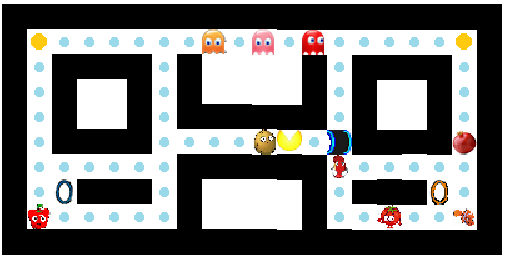
\includegraphics[width=0.75\linewidth]{map.png}
\caption{The system 2 map with the new blocs/fruits}
\label{fig:map}
\end{figure}

The fruits were created using the StaticTarget abstract class as eating a fruit will behave like eating a coin, exept that the eated fruit will trigger a new action. The action will, depending on the fruit, change the way Pacman behave for a certain period of time. Some of the fruits will change Pacman state, like the Bean or the Tomato. \\

\textbf{Fish}  This 'fruit' will make Pacman stops for 3 seconds. It will just change the speed of pacman to 0 for these 3 seconds. \\

\textbf{Grenade} I chose for this fruit to kill every ghosts in a range of 4 blocs and it doesn't care of walls. \\

\textbf{Pepper} The pepper will increase Pacman's speed to the maximum when eaten, so it will be set to 10 for 10 seconds. \\

\textbf{Potato} When eaten, the potato will increase ghost's speed to 7 for 5 seconds. \\

\textbf{Tomato} This fruit will change Pacman's state to INVINSIBLE for 4 seconds, in this mode Pacman cannot be eaten by the ghosts. So as this systems handle collisions in the WorkerProcess I added a condition that the ghost won't eat pacman if he is in this mode. The figure \ref{fig:invisible} shows pacman when he eats this fruit. \\

\begin{figure}[h!]
\centering

\includegraphics[width=0.2\linewidth]{invisible.png}
\caption{Pacman when in invinsible mode}
\label{fig:invisible}
\end{figure}

\textbf{RedBean} This very hot fruit will transform Pacman into Fire mode for 5 seconds, while in this state, he will throw Fireball each time he moves. The fireball kills every Ghost it met and it can cross multiple ghosts. Fireball is implemented with the DynamicTarget abstract class. The figure \ref{fig:fire} shows pacman when in fire mode. \\

\begin{figure}[h!]
\centering

\includegraphics[width=0.2\linewidth]{fire.png}
\caption{Pacman when in fire mode}
\label{fig:fire}
\end{figure}

The new map objects were implemented using a new abstract class that extends the MapObject abstract class. These objects will trigger some action when a Target is on it. \\

\textbf{Trap} This box will make the ghost or pacman's  speed to 0 for 3 seconds, it can only handle 1 target at a time, so if a ghost is stuck on the trap another ghost can cross it. \\

\textbf{Teleporter} There is 2 types of teleporter, an entry and a exit. When created a teleporter will be linked to another teleporter or liked to nothing, if the teleporter has a link it will move Pacman to the exit teleporter. On \wordlink{Figure}{fig:map} we can see the two types of teleporter, the blue on is the entry teleporter and the orange one is the exit. \\

\textbf{Bridge} The bridge can normally be used to make pacman cross crossroads, but in this systems there is none on the map, so in this case it will just block Pacman. For this block I created a new kind of state for DynamicTarget, the bridgeState, this state will have 3 main states: NOT\_ON, UNDER and ON. So it will be used to knwo if a target is not on a bridge, or under/on a bridge, collision between a ghost and pacman that are not on the same state won't happen. The  \wordlink{Figure}{fig:bridgeU} shows Pacman on a bridge and figure \wordlink{Figure}{fig:bridge} 'shows' pacman under a bridge.\\

\begin{figure}[h!]
\centering

\includegraphics[width=0.2\linewidth]{bridge4.png}
\caption{Pacman when on a bridge}
\label{fig:bridgeU}
\end{figure}

\begin{figure}[h!]
\centering

\includegraphics[width=0.2\linewidth]{bridge3.png}
\caption{Pacman when under a bridge}
\label{fig:bridge}
\end{figure}

The last commit for the implementation of the extension can be found here: \url{https://github.com/RemDec/pacman-system2/commit/5e6e4c46c404a25f3b98c9e9be61b890709eb71b}
\newpage
\subsection{System 3 (BOOSKO Sam)}

\subsubsection{Quality Improvement}

The title sounds weird in this section because we had to improve the quality in the previous step. Unfortunately for me, after reading the implementation and listening Robin speech about his work, I could notice that, it wouldn't be easy to add easily new features as demanded. I decided to rework few part of the system 3 based on what I did and saw in System 1.\\

Firstly, I changed the method based on a \textit{switch-case} in an object which creates a game element from a \textit{character} by a \textit{HashMap} where the keys are a \textit{Character} and the value an object, \textit{IElementBuilder}. The same way is used to create \textit{Cell} of the board. It's useful to bridge because bridges are not a game element but cell.\\

Secondly, I implemented a new object to manage collision with my new game element. Because, it wasn't my job to rework this system. I didn't change the previous collision detection. I added mine just to manage new collisions. It's based on a double \textit{HashMap} accesible by a couple of key (\textit{Class object}) to get an \textit{ICollisionAction} to perform the action on the game from this collision. \\

Finally, the last reworking is on \textit{MovingGameElement}. This class doesn't have any documentation and have an attribute \textit{speed}. It's quite difficult to understand the unit used for the speed and very diffult to \texttt{play} with it. Then, I decide to modify it to have a speed based on the unit, such as the number of cells traveled per second because usually, the speed unity follows the format such as $x$ unit of distance per $t$ unit of time. Also deleting code duplication from \textit{Pacman class} and \textit{Ghost class}, both extending \textit{MovingGameElement}.\\

\subsubsection{Features}

To be able to add new game element, a new abstract class is created, \textit{AExtensionElement}. This class provides a simply implementation to display an image for this game element. Also, to use this class such as a game element, it extends the main class \textit{GameElement}. Another little feature is the possibility to change the Pacman color to have a visualisation about his state.\\

\paragraph{Traps}

When Pacman goes on this game element, he is trapped for a random time between 1 and 4 seconds and turns red. This feature is implemented in \textit{pacman\_infd.Elements.ExtensionElements.TrapElement} (see Figure ~\ref{fig:system3Traps}).\\

\begin{figure}
\centering
    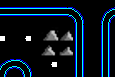
\includegraphics[width=.4\linewidth]{imgs/trapbefore.PNG}
    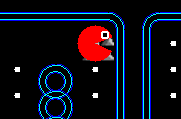
\includegraphics[width=.4\linewidth]{imgs/trapafter.PNG}
    \caption{System 3 - Traps}
    \label{fig:system3Traps}
\end{figure}

\paragraph{Teleportation} This game element is working by couple, because when the Pacman use a portal, he needs the output of this portal. In the rule chosen, only two portals can be created on a board. Also, a timer is used after the usage of a portal making the link broken during 2 seconds (see ~\ref{fig:system3Portals}). This feature is implemented in \textit{pacman\_infd.Elements.ExtensionElements.Telepo\\rterElement}. 

\begin{figure}
\centering
    
\includegraphics[width=.3\linewidth]{imgs/portal1.PNG}
    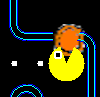
\includegraphics[width=.3\linewidth]{imgs/portal2.PNG}
    \caption{System 3 - Portals}
    \label{fig:system3Portals}
\end{figure}

\paragraph{Bridges} The bridges was the most complex feature to implement because it's not considered as a game element in this System. The best way to make this feature is to create a new kind of \textit{Cell}. This special cell assesses where is the \textit{MovingGameElement}, under or above the bridge. From this, it requires an override of default methods from \textit{Cell}. Two new lists are used, one with \textit{MovingGameElement} under the bridge and another one with \textit{MovingGameElement} above the bridge. Also, updates are made on the \textit{EventHandler} to let the collision checking assessing in the Cell object and on the \textit{MovingGameElement} to be able to know the current direction of the element. Thanks to these updates, the new Cell kind can manage how it wants the collision between game elements on itself and assesses as said where is the game element depending on his direction. This feature is mainly implemented in \textit{pacman\_infd.Game.BridgeCell} (see ~\ref{fig:system3Bridge}).

\begin{figure}
\centering
    
\includegraphics[width=.3\linewidth]{imgs/bridge1.PNG}
    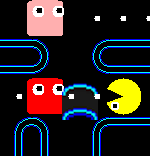
\includegraphics[width=.3\linewidth]{imgs/bridge2.PNG}
    \caption{System 3 - Bridges}
    \label{fig:system3Bridge}
\end{figure}

\paragraph{Grenade} The Grenade is implemented in \textit{pacman\_infd.Elements.ExtensionElements.GrenadeElement}. In the rule chose, the grenade kills all ghosts around in the maximum distance of 4 cases with a special specification. The grenade doesn't cross the walls. It means that a ghost can survive if he is protected by a wall. The main method for this is implemented on \textit{Cell} where a \textit{Breadth First Search} is implemented. The method takes two parameters, the Class (extends GameElement) searched in a maximum distance given as the second parameter (see ~\ref{fig:system3Grenade}.

\begin{figure}
\centering
    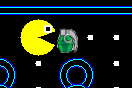
\includegraphics[width=.4\linewidth]{imgs/grenadeBoard.PNG}
    \caption{System 3 - Grenades}
    \label{fig:system3Grenade}
\end{figure}

\paragraph{Red Beans} The Red Bean, implemented in \textit{pacman\_infd.Elements.ExtensionElements.RedBeanElement}, is a special element. When Pacman eats this bean, Pacman is slown down by 50\% but he shoots 3 projectiles per second. These projectiles have the speed of $Pacman + 10$. Also, Pacman turns in dark red. The \textit{MovingGameElement} is used to create these projectile easily and a new collision is added in the \textit{CollisionMap} between \textit{Ghost} and \textit{Projectile} (see Figure ~\ref{fig:system3RedBeans}).

\begin{figure}
\centering
    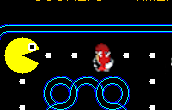
\includegraphics[width=.3\linewidth]{imgs/redBeanElement1.PNG}
    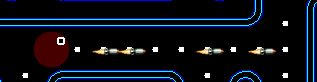
\includegraphics[width=.6\linewidth]{imgs/redBeanElement2.PNG}
    \caption{System 3 - Red Beans}
    \label{fig:system3RedBeans}
\end{figure}

\paragraph{Potato} The Potato, implemented in \textit{pacman\_infd.Elements.ExtensionElements.PotatoElement}, is a a simple element which increase the speed of all ghost on the board by 2 during a time. For this element, the visual information is done by ghosts which are faster than Pacman (see Figure ~\ref{fig:system3Potato}).

\begin{figure}
\centering
    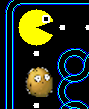
\includegraphics[width=.3\linewidth]{imgs/potato.PNG}
    \caption{System 3 - Potato}
    \label{fig:system3Potato}
\end{figure}

\paragraph{Fish} The fish is another simple element and the last, this one, implemented in \textit{pacman\_infd.Elements.ExtensionElements.Fish\\Element}, slows down the Pacman to a very slow speed and he turns cyan (see Figure ~\ref{fig:system3Fish}) . 

\begin{figure}
\centering
    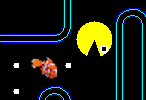
\includegraphics[width=.3\linewidth]{imgs/fish1.PNG}
    
\includegraphics[width=.3\linewidth]{imgs/fish2.PNG}
    \caption{System 3 - Fish}
    \label{fig:system3Fish}
\end{figure}

\paragraph{Elements Spawning System} All elements can be setup in the file map. During the game, two elements, the bridges and the teleporters don't spawn by the spawning system. This spawning system works such as for each pellet ate, there is 10\% that a random elements spawn on an empty \textit{cell}. This system is implement in the object \textit{GameWorld} on the method \textit{placeCherryOnRandomEmptyCell} already provided.


\newpage

\section{Quality evolution analysis}



\subsection{System 1 (Rémy)}

\indent From the extension development point of view, this implementation was really nice and easy to extend. The code was already well documented, and all is structured in a way it is quickly understandable. As the quality analysis at the beginning of the project mentionned, this is a quite good implementation that suffers really few drawbacks.
We lead firstly some statis analysis to get an overview of how the implementation evolved. 


\begin{figure}[h]
\centering
\includegraphics[width=0.7\linewidth]{S1-designite_final}
\caption{Results from Designite for final system 2}
\label{fig:S1_designite_final}
\end{figure}

\newpage

We observe in \wordlink{Figure}{fig:S1_designite_final} that the system has consequently increased in size, almost doubled in mulitple counting metrics (LOC, number of classes/methods). The increasing size of the code lead to some new bad smells, but also avoided some previously present. Some metrics like magic numbers seem still (41 now, 39 previously), but actually this is not the case considering the implementation almost doubled in size. An metric that increased a lot is the unutulized abstraction, growing from 4 to 55. But some important ones also go better, like the number of cyclic dependencies that lowered from 5 to 1.\\

Wan can no more use CodeMR with this system because we need a license due to the increased size. It is hard to found an equivalent that retrieves the same metrics. However, we used some built-in Intellij to perform complexity analysis. Results are depicted by \wordlink{Figure}{fig:S1_compl_final}. The average cyclomatic complexity ranges from 1 to 1.70, there is no strong variation from a package to another that could indicate some ``super methods". However, some classes have a high weighted method complexity, these outliers are in central classes like \texttt{Level} and \texttt{Board}.\\

\begin{figure}[h]
\centering
\includegraphics[width=\linewidth]{S1-compl_final}
\caption{Complexity metrics at package and class levels for final system 2}
\label{fig:S1_compl_final}
\end{figure}

\vspace{0.8cm}

The \wordlink{Figure}{fig:S1_depmatrix_final} confirms what Designite told us : the new written classes under \texttt{specialpellet} and \texttt{specialbox} packages didn't introduce new cycles in the system, preserving its design quality. There are still some big classes like \texttt{Level} implied in a lot of dependencies, but sometimes it's impossible to avoid it. \\

Another aspect is the javadoc coverage, that was initially very good. For the similar tabular than \wordlink{Figure}{fig:S1_javadoc_final}, we had in average 100\% (class coverage), 82\% (fields coverage), 232 lines of javadoc and 84\% (methods coverage). It looks like the documentation quality lowered, but we have to consider that the package structure changed. We also notice that the average number of lines increased, meaning that what had absolutly to be documented is well documented (some non relevant fields may have been omitted leading to the observed lowering).

\newpage

\vspace{0.2cm}

\begin{figure}[h]
\centering
\includegraphics[width=0.95\linewidth]{S1-depmatrix_final}
\caption{Dependency matrix for final system 2}
\label{fig:S1_depmatrix_final}
\end{figure}

\vspace{0.3cm}

\begin{figure}[h]
\centering
\includegraphics[width=0.52\linewidth]{S1-doc_final}
\caption{Results for javadoc coverage for final system 2}
\label{fig:S1_javadoc_final}
\end{figure}

\newpage

We use the test coverage provided by Intellij to analyze which part of the code are not under test coverage. Global results are given by \wordlink{Figure}{fig:S1_testcover_final}. We observe that the coverage stayed good, as new tests have been written to test the extension features. The 57 tests available (45 previously) pass without any problem.\\

\begin{figure}[h]
\centering
\includegraphics[width=0.8\linewidth]{S1-testcover_final}
\caption{Results for test coverage for final system 2}
\label{fig:S1_testcover_final}
\end{figure}

\subsection{System 2 (Robin)}

\subsubsection{Generalities}

This system is a mess, Rémy improved it but the system was too bad to begin with, everything could have been changed but it would have taken too much time. The way the collisions are handled is, I think, bad, it's not really clear how we have to create new collision type. Also creating or modify the map is dreadful, it was a pain to change the map, but of course changing that would have taken a lot of time. Creating new type of object is also not that easy because we have to create new Containers, ... And WorkerProcess is, in my mind, a mess in general, it doesn't really respect object oriented programming, everything is compared with else-if with a lot of Feature Envy, everything could have been reworked to make it clearer and simpler to update. But still tanks to Rémy this system is clearer than before.

\subsubsection{Static Analysis}
\subsubsection{Code Metrics (CodeMR)}
  CodeMR was used before to anylise the system but now we cannot do it because of the free version, the system is now too big for the free trial. We couldn't afford to buy the full version.

\subsubsection{Compliance & bad smells (PMD, Designite)} 

\textbf{PMD} The \wordlink{Figure}{fig:pmd} shows the results of the PMD analysis, we can see that there is 1880 violations.

\textbf{Designite} The \wordlink{Figure}{fig:designite} shows the results of the Designite analysis, there is still a lot of code smels, like 12 cyclic dependencies, 7 complex method, 1 Feature Envy and 162 magic numbers.

\begin{figure}[h!]
\centering
\includegraphics[width=0.75\linewidth]{pmdFinal.png}
\caption{PMD results for system 2}
\label{fig:pmd}
\end{figure}

\begin{figure}[h!]
\centering
\includegraphics[width=0.75\linewidth]{designiteFinal.png}
\caption{Designite result for system 2}
\label{fig:designite}
\end{figure}

\subsubsection{Test coverage (Intellij built-in tool)}

The following figures \ref{fig:acov},  and \ref{fig:acov2} shows the test coverage. All the tests passed and almost all the code is covered. We can see that 96\% of the classes were tested and 71\% of the code line. 
\newpage

\begin{figure}[h!]
\centering
\includegraphics[width=0.75\linewidth]{testCovS2.png}
\caption{System 2 test coverage}
\label{fig:acov}
\end{figure}

\begin{figure}[h!]
\centering
\includegraphics[width=0.75\linewidth]{testCov2S2.png}
\caption{System 2 test coverage}
\label{fig:acov2}
\end{figure}
\newpage

\subsection{System 3 (BOOSKO Sam)}

\subsubsection{Generalities}

The personal view is that a lot of improvements can be done, but it should mean, rework all the system. This system, is, according to me, not good. A lot of parts are not clear, not easy to modify, or to update without changing a huge part of it. It would be too long to enumerate all of these problems seen. But few of them are, 1) the merging between, the controller, the visual and the core (model), 2) using not logical value for attributes as the previous speed in the object \textit{MovingGameElement}, increasing this value gave the effect of slowing down the GameElement, 3) the class \textit{Wall}, don't need to explain, just opening it make us understand and many more problems could be said.\\

\subsubsection{Static Analysis}

\paragraph{Bad smells (Designite)} 
With Designite, we observe that there are 229 magic numbers (see Figure ~\ref{fig:system3EndStepDesignite}), corresponding in the implemention of the default elements drawing method. In general, the system is doing well. 

\begin{figure}
\centering
    \includegraphics[width=\linewidth]{imgs/system3LastStepDesignite.PNG}
    \caption{System 3 - Designite Output}
    \label{fig:system3EndStepDesignite}
\end{figure}

\paragraph{Javadoc Coverage (MetricsReloaded)}
We observe that the javadoc coverage should be improved (see Table ~\ref{tab:system3EndStepJavaDoc}).

\begin{table}
\centering
    \includegraphics[width=\linewidth]{imgs/JavaDocCoverageS3.PNG}
    \caption{System 3 - Javadoc Coverage}
    \label{tab:system3EndStepJavaDoc}
\end{table}

\subsubsection{Dynamic Analysis}

\paragraph{Running tests \& Test Coverage (IntelliJ Build-Run)} By running the tests provided and new tests added, 28 tests of 28 passed. Furthermore, the project is quite well covered by tests (see Table ~\ref{tab:system3EndStepTestCoverage}). Anyway, some improvements could be done.

\begin{table}
\centering
    \includegraphics[width=\linewidth]{imgs/system3lastStepTestCover.PNG}
    \caption{System 3 - Test Coverage}
    \label{tab:system3EndStepTestCoverage}
\end{table}



 
\end{document}